\documentclass[12pt,a4paper,openright,twoside]{report}

\usepackage[italian]{babel}

\usepackage[latin1]{inputenc}
% libreria per impostare il documento
\usepackage{fancyhdr}
% libreria per avere l'indentazione
% all'inizio dei capitoli, ...
\usepackage{indentfirst}
% libreria per mostrare le etichette
%\usepackage{showkeys}
% libreria per inserire grafici
\usepackage{graphicx}
% libreria per utilizzare font
%   particolari ad esempio
%   \textsc{}

\usepackage{listings}

\usepackage{newlfont}
% librerie matematiche
\usepackage{amssymb}
\usepackage{amsmath}
\usepackage{latexsym}
\usepackage{amsthm}

\oddsidemargin=30pt \evensidemargin=20pt%impostano i margini
\hyphenation{sil-la-ba-zio-ne pa-ren-te-si}%serve per 

% comandi per l'impostazione
%   della pagina, vedi il manuale
%   della libreria fancyhdr
%   per ulteriori delucidazioni
\pagestyle{fancy}\addtolength{\headwidth}{20pt}
\renewcommand{\chaptermark}[1]{\markboth{\thechapter.\ #1}{}}
\renewcommand{\sectionmark}[1]{\markright{\thesection \ #1}{}}
\rhead[\fancyplain{}{\bfseries\leftmark}]{\fancyplain{}{\bfseries\thepage}}
\cfoot{}
\linespread{1.3} %comando per impostare l'interlinea
% definisce nuovi comandi

\begin{document}

\include{frontespizio}
\clearpage{\pagestyle{empty}\cleardoublepage}
\begin{titlepage}                       %crea un ambiente libero da vincoli
                                        %   di margini e grandezza caratteri:
                                        %   si pu\`o modificare quello che si
                                        %   vuole, tanto fuori da questo
                                        %   ambiente tutto viene ristabilito
\thispagestyle{empty}                   %elimina il numero della pagina
\topmargin=6.5cm                        %imposta il margina superiore a 6.5cm
\raggedleft                             %incolonna la scrittura a destra
\large                                  %aumenta la grandezza del carattere
                                        %   a 14pt
\em                                     %emfatizza (corsivo) il carattere
Alla mia famiglia.                      
\newpage                                %va in una pagina nuova
\clearpage{\pagestyle{empty}\cleardoublepage}
\end{titlepage}
\clearpage{\pagestyle{empty}\cleardoublepage}
\chapter*{Introduzione}
\addcontentsline{toc}{chapter}{Introduzione}
Nell'ambito dello studio dei plasmi generati tramite scariche elettriche si rivela necessario catturare gli spettri generati da suddette interazioni per studiarne diverse propriet� quali composizione e temperatura. Per effettuare tali misurazioni sono necessari due strumenti: un monocromatore che scomponga e rifletta la fonte di luce in input e una fotocamera che catturi l'immagine dello spettro. \\
Risulta quindi necessaria un'interfaccia utente in grado di controllare simultaneamente i due strumenti in modo da facilitare il percorso di acquisizione e manipolazione degli spettri. Lo scopo della tesi � implementare l'interfaccia richiesta attraverso il linguaggio di programmazione grafica LabVIEW, con l'ausilio delle API dei due strumenti.\\
� presente un progetto preesistente che realizza l'interfaccia di controllo del monocromatore e di una fotocamera non intensificata. A partire da questo progetto se ne � realizzato uno nuovo che riutilizza alcune parti del precedente, considerando lo stesso monocromatore e una nuova fotocamera intensificata.\\
A partire quindi dal programma esistente si � effettuato uno studio dello stesso per poterlo cos� adattare alla nuova fotocamera. Dopo un primo tentativo di riutilizzo e refactoring si � preferito realizzare un programma ex novo, modificando anche alcuni elementi dell'interfaccia grafica. Chiaramente si sono mantenuti alcuni elementi, in particolare quelli legati al monocromatore, dal momento che lo strumento � rimasto lo stesso cos� come le librerie ad esso associate.
%non numera l'ultima pagina sinistra
\clearpage{\pagestyle{empty}\cleardoublepage}

\pagenumbering{roman}
%indice
\tableofcontents                        %crea l'indice

%non numera l'ultima pagina sinistra
\clearpage{\pagestyle{empty}\cleardoublepage}
\listoffigures                          %crea l'elenco delle figure
%non numera l'ultima pagina sinistra
\clearpage{\pagestyle{empty}\cleardoublepage}

\pagenumbering{arabic} 

\chapter{Documento dei requisiti}
\thispagestyle{empty}
%\lhead[\fancyplain{}{\bfseries\thepage}]{\fancyplain{}{\bfseries\rightmark}}

Si descrive nelle seguenti sezioni la specifica dei requisiti del sistema software che si intende sviluppare.

\section{Scopo}
Come accennato nell'introduzione si rende necessaria la realizzazione di una nuova interfaccia che possa controllare simultaneamente il monocromatore HR640 e la fotocamera intensificata 4Picos. Il precedente programma aveva la capacit� di controllare lo stesso monocromatore ma una diversa fotocamera, SensiCam (version 3.0).

\section{Descrizione generale}
L'utente, attraverso il programma da progettare, deve poter controllare sia il monocromatore che la fotocamera intensificata. � importante che questi due strumenti possano essere controllati simultaneamente poich� le loro funzioni sono strettamente legate: il monocromatore genera un determinato spettro attraverso la sua struttura interna e la fotocamera deve poter catturare tale spettro il pi� precisamente possibile.

\subsection{Funzioni del prodotto}
Attraverso il programma deve essere possibile inizializzare le principali caratteristiche del monocromatore in base alle esigenze dell'utente: grating, lunghezza d'onda e slit (fessura?) di entrata. Deve anche essere possibile settare e modificare le impostazioni della fotocamera, compatibilmente con le funzioni messe a disposizione tramite le API della stessa. 

\subsection{Caratteristiche utente}
Il progetto da realizzare viene utilizzato da professori e dottorandi nell'ambito di ricerca ???. � necessario trovare un punto di equilibrio tra le esigenze dell'utente e i vincoli di programmazione.

\section{Requisiti specifici}

\subsection{Requisiti dell'interfaccia utente}
L'interfaccia deve risultare il pi� intuitiva possibile, per questo si deve cercare di mantenere un minimo di omogeneit� con il programma passato. Devono infatti coesistere nella stessa finestra sia i controlli per il monocromatore che quelli per la fotocamera.\\Vediamo quali sono i requisiti specifici per i due strumenti.

\begin{description}
  \item[Monocromatore] Per quanto riguarda la parte di interfaccia che permette di impostare correttamente il monocromatore � necessario poter modificare il grating (1200 o 2400) e la calibrazione di correzione relativa. Si deve anche poter modificare la slit di entrata e la lunghezza d'onda;
  \item[Fotocamera] La parte di interfaccia che concerne la fotocamera intensificata deve contenere i seguenti parametri:
	\begin{itemize}
\item MCP Gain Voltage: guadagno di tensione in volt tra 600 e 950
\item Exposure Time: tempo di esposizione, deve essere maggiore di zero e si deve poter specificare l'unit� di misura
\item Delay: ritardo in secondi dell'acquisizione dell'immagine
\item Frames to accumulate: numero di immagini da acquisire
\item Trigger Source: -Trig per far scattare l'otturatore esternamente attraverso l'input di trigger negativo collegato elettricamente ad un segnale, Fsync per far scattare l'otturatore internamente dal segnale Fsync
\item Gate Control: interno, l'input di controllo dell'otturatore � connesso internamente all'output IntGtP che pu� essere usato per scopi di controllo o trigger, o esterno, l'input di controllo dell'otturatore � collegato al connettore in input di ExtGtP
\item Start Option: Cold Start, non ci sono parametri pregressi da utilizzare, Warm Start, dopo il riavvio della fotocamera si chiede all'utente se si devono caricare i parametri usati precedentemente, Auto Warm Start, dopo il riavvio della fotocamera vengono caricati i parametri usati in precedenza senza la conferma da parte dell'utente
\item Detector: per specificare l'area attiva del chip CCD, frame intero, binning 2x2 oppure ROI (Region of Interest, solo 1/3 dell'area complessiva)
\item Digitalizer Mode: acquisizione dell'immagine con una precisione di 8 o 14 bit per pixel
\item CCD Gain: automatico oppure settabile manualmente (in dB)
\item Trigger Mode: trigger diretto (ad ogni segnale di trigger far� scattare l'otturatore) oppure singolo (in questo caso deve essere possibile inserire il numero di trigger per frame)
\item Modalit� di acquisizione dell'immagine: Single Exposure per catturare una sola immagine, Live Mode per acquisire immagini in modo continuo;
\end{itemize}
\end{description}
Devono anche essere presenti dei comandi per il post-processing e l'analisi delle immagini acquisite. Come nel progetto preesistente � necessario visualizzare lo spettro in un grafico che abbia nell'asse orizzontale il range di lunghezza d'onda osservato e nell'asse verticale (cosa?). Inoltre deve essere possibile sottrarre un background acquisito in precedenza ed effettuare altri calcoli sullo spettro. Alla fine delle operazioni qualora ce ne sia la possibilit�, si deve poter salvare i dati in un file di testo che tenga traccia dei valori calcolati per visualizzare lo spettro.

\subsection{Linguaggio di programmazione}
Il linguaggio di programmazione da utilizzare per realizzare il progetto richiesto � LabVIEW.\\ LabVIEW � un linguaggio di programmazione grafica (G - Graphical Programming Language) che utilizza un modello a flusso di dati invece di linee sequenziali di codice testuale, permettendo di scrivere codice funzionale utilizzando un layout grafico che assomiglia a un diagramma di flusso. \\
L'ambiente di programmazione LabVIEW presenta due principali finestre di lavoro: front panel e block diagram. 
\begin{description}
\item[Front Panel]Finestra in cui si visualizza e si modifica l'interfaccia utente. Sono disponibili diversi stili e comandi per l'interazione con l'utente.
\item[Block Diagram]Finestra in cui si compone il codice a blocchi, controlli, indicatori, subVI e moltre alte componenti. Da tale finestra � possibile effettuare il debug del codice e controllare il contenuto delle variabili.
\end{description}
Le strutture principali utilizzate nel codice sono cicli, while e for, e case structure, che funzionano come if o switch. Per mantenere il valore delle variabili e condividerle con altre strutture si usano fili che le interconnettono. Elementi fondamentali nel linguaggio di programmazione grafica sono controlli e indicatori: i controlli permettono all'utente di inserire o modificare i dati, mentre gli indicatori consentono di visualizzare lo stato delle variabili.
\chapter{Analisi del progetto preesistente}
\thispagestyle{empty}
%\lhead[\fancyplain{}{\bfseries\thepage}]{\fancyplain{}{\bfseries\rightmark}} 

\section{Breve descrizione degli strumenti coinvolti}

\subsection{Monocromatore}
Un monocromatore \`e un dispositivo che scompone un singolo fascio di luce policromatica in pi\`u fasci di luce monocromatica (che contiene cio\`e onde di una sola frequenza), permettendo cos\`i di analizzare l'intensit\`a in funzione della lunghezza d'onda.\\
Nello strumento la luce policromatica entra da una fessura; tramite un sistema ottico viene inviata su un reticolo di diffrazione o ad un prisma che scompone il fascio. Una seconda fenditura raccoglie poi il fascio di una determinata lunghezza d'onda.\\
In questo progetto si considera un monocromatore Jobin-Yvon HR460. La luce che entra dalla fessura viene rifratta (?) due volte attraverso due lenti tra cui \`e interposta una griglia che scompone il fascio di luce. 

\subsection{Fotocamera}
Una fotocamera intensificata \`e una fotocamera che al posto della pellicola fotosensibile utilizza un sensore (CCD) in grado di catturare l'immagine e trasformarla in un segnale elettrico di tipo analogico. Gli impulsi elettrici vengono convertiti in digitale da un convertitore analogico/digitale in un chip di elaborazione esterno al sensore. Viene quindi generato un flusso di dati digitali atti ad essere immagazzinati in vari formati su supporto di memoria.\\
Il CCD (Charged-Coupled Device) \`e un dispositivo attraverso il quale si ottiene un segnale elettrico in uscita, in seguito a una sequenza temporizzata di impulsi, grazie al quale \`e possibile ricostruire la matrice di pixel che compongono l'immagine proiettata sulla superficie del CCD stesso. Questa informazione pu\`o essere usata come segnale analogico, e quindi essere usata per riprodurre l'immagine su un monitor, oppure pu\`o essere convertita in formato digitale.

\section{Principali funzioni}
Il progetto preesistente ha le stesse funzioni del nuovo programma richieste, con alcune eccezioni per quanto riguarda la fotocamera. Quella utilizzata precedentemente presentava alcune funzioni che la nuova fotocamera non mette a disposizione. Ad ogni modo si descriver\`a il progetto cercando di evidenziare le funzionalit\`a che necessitano di essere abbandonate a causa della diversit\`a dei due strumenti.\\
L'interfaccia non presenta alcuna divisione tra i controlli dei due strumenti e si possono quindi controllare simultaneamente senza alcuna distinzione. � chiaro che lo strumento che ha priorit� in fase di inizializzazione � il monocromatore, in quanto composto da elementi fisici che devono essere riportati con movimenti meccanici ad una posizione di dafault; solo una volta che le lenti e la griglia all'interno dello strumento si trovano nella posizione iniziale � possibile cominciare ad utilizzare il programma.

\subsection{Monocromatore}
I comandi presenti per controllare il monocromatore sono gli stessi richiesti nel nuovo progetto: selezione del grating (e rispettive calibrazioni per correggere eventuali errori), impostazione della lunghezza d'onda e slit di entrata. Sono inoltre presenti dei led che mostrano eventuali errori: un errore generico in fase di inizializzazione, lunghezza d'onda inserita errata e superamento dei limiti dei valori consentiti.

\subsection{Fotocamera}
Per quanto riguarda la fotocamera si distingue fra acquisizione singola o continua ed � possibile inserire tempo di esposizione e ritardo di acquisizione dell'immagine. Si pu� inoltre scegliere un valore specifico di binning, fino a 1/16 per il binning verticale e fino a 1/8 per il binning orizzontale. Viene anche segnalato un'eventuale caso di saturazione con un calcolo successivo alla foto.

\subsection{Altre opzioni}
� possibile effettuare delle operazioni non collegate direttamente ai due strumenti. Oltre a visualizzare l'immagine cos� come � stata presa, � anche possibile visualizzare lo spettro corrispondente in seguito a determinati calcoli. Su tale spettro si possono richiedere alcune informazioni quali l'integrale su un certo intervallo della lunghezza d'onda, il numero di picchi rilevati al di sopra di una certa soglia; viene inoltre mostrato, senza bisogno di chiederlo, il valore del picco pi� alto alla lunghezza d'onda corrispondente e la FWHM (Full Width at Half Maximum), che corrisponde alla differenza fra i valori assunti dalla variabile indipendente lunghezza d'onda quando la variabile dipendente y (?) � pari a met� del suo valore massimo.
� disponibile un comando per l'acquisizione del background (legato per� alla fotocamera): infatti nel caso in cui lo spettro venga generato in un ambiente (visivamente) ``rumoroso'' si pu� successivamente utilizzare il suddetto dato per sottrarlo a immagini successive, in modo da renderle il pi� chiare possibile.

\section {Codice del progetto preesistente}
Si analizza nella seguenti sezioni il codice del progetto preesistente, al fine di giustificare la scelta di progettazione fatta successivamente. La descrizione del codice si articola fra analisi del front panel e del block diagram, che sono i due ambienti di programmazione principale del linguaggio \emph{LabVIEW}.

\subsection{Front Panel}
\textbf{------- inserire foto front panel -------}
Il front panel � diviso in blocchi ideali che non dividono veramente il codice ma danno all'utente tale impressione.\\
In alto si trova una tab control che mostra, a seconda della selezione, l'immagine acquisita oppure lo spettro; per visualizzare lo spettro dopo aver l'immagine e viceversa � necessario riacquisire i dati. Nella sezione dedicata allo spettro sono presenti tre indicatori che mostrano il valore del picco massimo alla lunghezza d'onda corrispondente e il valore della FWHM in mm.\\
La prima fascia di pannelli � composta da tre parti. La prima contiene un bottone booleano con cui si richiede il numero di picchi oltre una certa soglia, i cui valori vengono visualizzati in indicatori di array. La seconda permette di inserire gli estremi di un intervallo di lunghezza d'onda e di richiederne, attraverso un bottone booleano, l'integrale. La terza parte non � delimitata da un vero e proprio pannello ma contiene due indicatori di versione (main e boot) del monocromatore, un indicatore della acquisizioni fino a quel momento e il bottone booleano di uscita.\\
La seconda fascia � divisa in due parti. La prima, dedicata alla fotocamera, contiene un bottone booleano per acquisizione singola e uno per quella continua, due controlli e rispettivi indicatori per ritardo ed esposizione, due quadranti per impostare il binning verticale e orizzontale, un led di indicazione di un'eventuale saturazione e un controllo per inserire il numero di pixel su cui fare la media per generare lo spettro. La seconda parte contiene invece controlli e indicatori per il monocromatore: bottone booleano per il grating (1200 o 2400) e rispettivi controlli per inserire la calibrazione in entrambi i casi, un controllo per inserire la lunghezza d'onda e uno per la slit di entrata, due indicatori per mostrarne i valori reali, e tre led che indicano se il monocromatore � stato correttamente inizializzato o se sono presenti errori generici, lunghezza d'onda non valida e superamento dei limiti consentiti.\\
La terza fascia � divisa in quattro parti. Nella prima c'� la possibilit� di salvare i dati con un file path predefinito (calcolato secondo le impostazioni del programma) oppure da inserire manualmente. Nella seconda parte � possibile selezionare il modo di acquisizione della foto, via software (impostazione di dafault), trigger esterno al fronte di salita o trigger esterno al fronte di discesa; con un bottone booleano si modifica la modalit� e un led indica se il programma � in attesa di un trigger. La quarte parte indica la temperatura del CCD e della board (?) della camera.

\subsection{Block Diagram}
\textbf{------- inserire foto block diagram -------}
Il block diagram � composto di una macro flat sequence (sequenza che forza il flusso dei dati in una determinata sequenza scelta dal programmatore) divisa in tre blocchi: il primo che delimita l'inizializzazione degli strumenti, il secondo contiene il codice principale del programma, e il terzo chiude in modo corretto la fotocamera.

\subsubsection{Primo blocco}
Questo blocco � dedicato principalmente all'inizializzazione del monocromatore. � presente un'ulteriore flat sequence di 3 blocchi. Nel primo viene invocato il subVI \emph{StartUp.vi} che inizializza il monocromatore e riporta i componenti interni alle posizioni di default. Questo subVI restituisce in uscita una lista di errori e le informazioni riguardo il numero di versione del monocromatore. Nel secondo blocco � presente un timer che mette in pausa il programma per 1 secondo e nel terzo blocco il led di inizializzazione viene commutato a vero per indicare l'avvenuta inizializzazione dello strumento.\\
Oltre al subVI del monocromatore ne vengono chiamati altri due che riguardano la fotocamera: \emph{SCSetBoard.vi} e \emph{SCSetMode.vi} servono per inizializzare la scheda della fotocamera e danno in uscita un cluster che contiene eventuali errori.\\
Al di fuori di questa flat sequence � presente del codice per caricare un file che contiene dati utilizzati successivamente per compiere alcuni calcoli.

\subsubsection{Secondo blocco}
Questo blocco � composto da un ciclo con al suo interno un'altra flat sequence. Il ciclo while � necessario per rendere il programma sensibile in qualsiasi momento al cambiamento di qualche impostazione (switch di un bottone booleano o del valore di un controllo); viene bloccato solo quando viene invocato lo stop, con l'apposito bottone. La flat sequence all'interno del ciclo � divisa in cinque blocchi che si descrivono qui di seguito.
\begin{itemize}
	\item Primo blocco. Contiene un ulteriore ciclo while. All'interno di questo ciclo troviamo alcune case structure che vengono eseguite solo nel caso in cui il controllo a cui sono associate assume un certo valore. La case structure associata al bottone booleano \textit{Save} permette di salvare i dati qualora questo venga premuto; il nome con cui viene salvato il file viene costruito dalla funzione di concatenazione di stringhe che ha in ingresso le impostazioni caratteristiche del programma nel momento in cui si decide di salvare. La case structure associata al bottone booleano \textit{Waveform Integral} calcola, se richiesto, l'integrale della lunghezza d'onda su un intervallo specificato. � presente una case structure associata a un'ulteriore bottone booleano di \textit{Save} che per� al suo interno manca della funzione di concatenazione, il path del file viene infatti inserito manualmente dall'utente in un apposito controllo. Nella case structure associata al controllo booleano \textit{Load Coeff} � presente una funzione per caricare un file con certi valori che possono essere usati successivamente nel programma. La case structure associata al controllo \textit{Peak Detector} calcola, attraverso il subVI \emph{Waveform Peak Detection.vi} il numero di picchi sopra una certa soglia con relativa lunghezza d'onda. Un'altra case structure associata al controllo booleano \textit{Grating} discrimina in base al valore del grating il valore da dare in ingresso al monocromatore. � presente infatti un'altra flat sequence divisa in quattro blocchi: nel primo viene invocato il subVI \emph{Port \& Grating.vi} per impostare il grating e il tipo di input del monocromatore, nel secondo attraverso il subVI \emph{Spectral GOTO.vi} si richiede al monocromatore di portare i componenti interni alle posizioni inserite dell'utente, nel terzo con il subVI \emph{Slits.vi} si imposta la slit di entrata, nel quarto il subVI \emph{Spectral Position.vi} restituisce la lunghezza d'onda effettiva a cui si trova il monocromatore.
	\item Secondo blocco. Completamente dedicato alla fotocamera. Dapprima vengono invocati i subVI \emph{SCStopCoC.vi} e \emph{SCGetStatus.vi} che restituiscono le informazioni di temperatura e di due componenti della fotocamera. In seguito alla costruzione di un cluster contente le impostazioni della fotocamera vengono invocati i subVI \emph{New Delay and exposure formatter.vi} per la formattazione del ritardo e del tempo di esposizione e \emph{SCSetNewCoC.vi} per inviare le impostazioni alla fotocamera. L'ultimo subVI chiamato � \emph{SCRun.vi} che, come suggerisce il nome stesso, fa partire la fotocamera.
	\item Terzo blocco. Anche questo riguarda solo la fotocamera e contiene tre subVI. Il primo \emph{SCGetImageStatus.vi} � wrappato all'interno di un ciclo while ed � il subVI che permette l'acquisizione vera e proprio dell'immagine. I dati acquisiti con questo subVI vengono poi passati al subVI successivo, \emph{SCGetImageSize.vi}, che restituisce le dimensioni in pixel dell'immagine. I dati che escono da questo subVI sono date in ingresso al successivo, \emph{SCGet12BitImage}, che restituisce l'immagine. Infine attraverso una case structure viene commutato il valore del led \textit{Saturation} in base al valore dei pixel risultati dall'ultimo subVI.
	\item Quarto blocco. Contiene una case structure associata al bottone booleano \textit{Grating} che calcola i valori da inserire nel grafico che mostra lo spettro. Tali calcoli vengono effettuati a partire dalla dimensione della foto (che varia se � stato utilizzato un particolare binning) e dal valore di ogni pixel; per prima cosa vengono calcolati i valori delle lunghezze d'onda da visualizzare sull'asse orizzontale del grafico, in modo speculare rispetto al centro dell'immagine, e in seguito viene calcolata una media di un certo numero di pixel (dati dal controllo \textit{Pixel to Average}) per i valori da visualizzare nell'asse verticale del grafico.
	\textbf{Mancano le formule da inserire}
In questa case structure ne � contenuta anche una associata al bottone booleano \textit{Subtract Dark} per eliminare un eventuale background acquisito in precedenza. 
	\item Quinto blocco. Consente al programma di visualizzare l'immagine o lo spettro, in base alla scelta dell'utente. In questo punto del programma vengono anche effettuati i calcoli dei valori \textit{FWHM}, \textit{Max Peak} e \textit{WL}.
\end{itemize}

\subsubsection{Terzo blocco}
Questo blocco contiene solamente il subVI \emph{SCSetMode.vi} che termina il funzionamento della fotocamera attraverso il valore adatto di un enumerativo. Anche se quest'ultimo passaggio potrebbe sembrare inutile � sempre bene ricordare che tutti i programmi che vengono eseguiti impiegano un certo numero di risorse: utilizzare le giuste funzioni o i giusti subVI di chiusura anche per gli strumenti coinvolti permette di liberare le risorse impegnate senza scansando il rischio di un uso ridondante della memoria.

\section{Considerazioni sul progetto a livello di programmazione}
L'analisi del codice gi� esistente si � resa necessaria in quanto uno dei due strumenti, in particolare il monocromatore, non � stato sostituito. Ad una prima lettura superficiale il codice risulta funzionante. Tuttavia 
\chapter{Fase preliminare alla realizzazione del progetto}
\thispagestyle{empty}

Prima della realizzazione del progetto per controllare entrambi gli strumenti, si � optato per la scrittura di due progetti separati. In questo modo � stato possibile verificare la versione del codice pi� efficacie per ogni strumento, cos� da poter unire in seguito le due logiche, evitando conflitti.

\section{Fotocamera}

Per entrare in confidenza con il linguaggio di programmazione grafico LabVIEW e con lo strumento, si � reso necessario partire da un esempio fornito con le API LabVIEW legate alla nuova fotocamera intensificata \cite{miseAnServiceCamera}.

\subsection{Breve descrizione dello strumento}
La fotocamera intensificata per cui si deve scrivere il programma che la controlli � la 4 Picos con CCD intensificato di Stanford Computer Optics, Inc.

\subsection{Descrizione dell'esempio fornito}

L'esempio fornito � molto semplice e non contiene tutte le opzioni disponibili per la fotocamera. Analizziamo come fatto in precedenza i due componenti principali del programma: front panel e block diagram.

\subsubsection{Front Panel}
\begin{figure} [h]
	\centering
	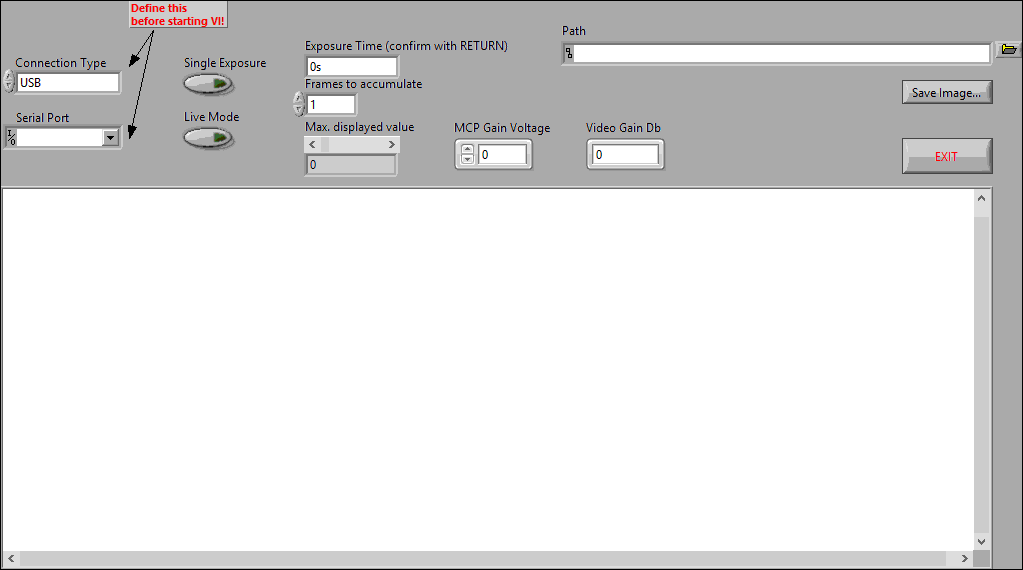
\includegraphics[width=\linewidth]{img/SCOexample_fp.png}
	\caption{Front Panel del progetto per sola fotocamera}
	\label{fig:midProj_camera_fp}
\end{figure}
Nel front panel in figura \ref{fig:midProj_camera_fp} possiamo vedere due controlli che � obbligatorio definire prima della partenza del VI, e sono il tipo di connessione \textit{Connection Type} e la porta seriale \textit{Serial Port} nel caso in cui il tipo di connessione sia \textit{Analog}. � infatti permesso scegliere fra tre tipi di connessione allo strumento: \textit{USB} (che � la connessione usata nel nostro caso), \textit{CameraLink} o \textit{Analog}. A fianco di questi due controlli troviamo due bottoni booleani per acquisire immagini in un singolo frame oppure in modo continuo. � poi possibile inserire il tempo di esposizione \textit{Exposure Time}, il numero di frame da catturare \textit{Frames to accumulate}, e modificare il valore \textit{Max. displayed value} del fondo scala. Un indicatore di immagine rende possibile la visualizzazione dell'immagine e un bottone booleano permette di salvare l'immagine. Infine troviamo un controllo per terminare il programma.

\subsubsection{Block Diagram}
\begin{figure} [h]
	\centering
	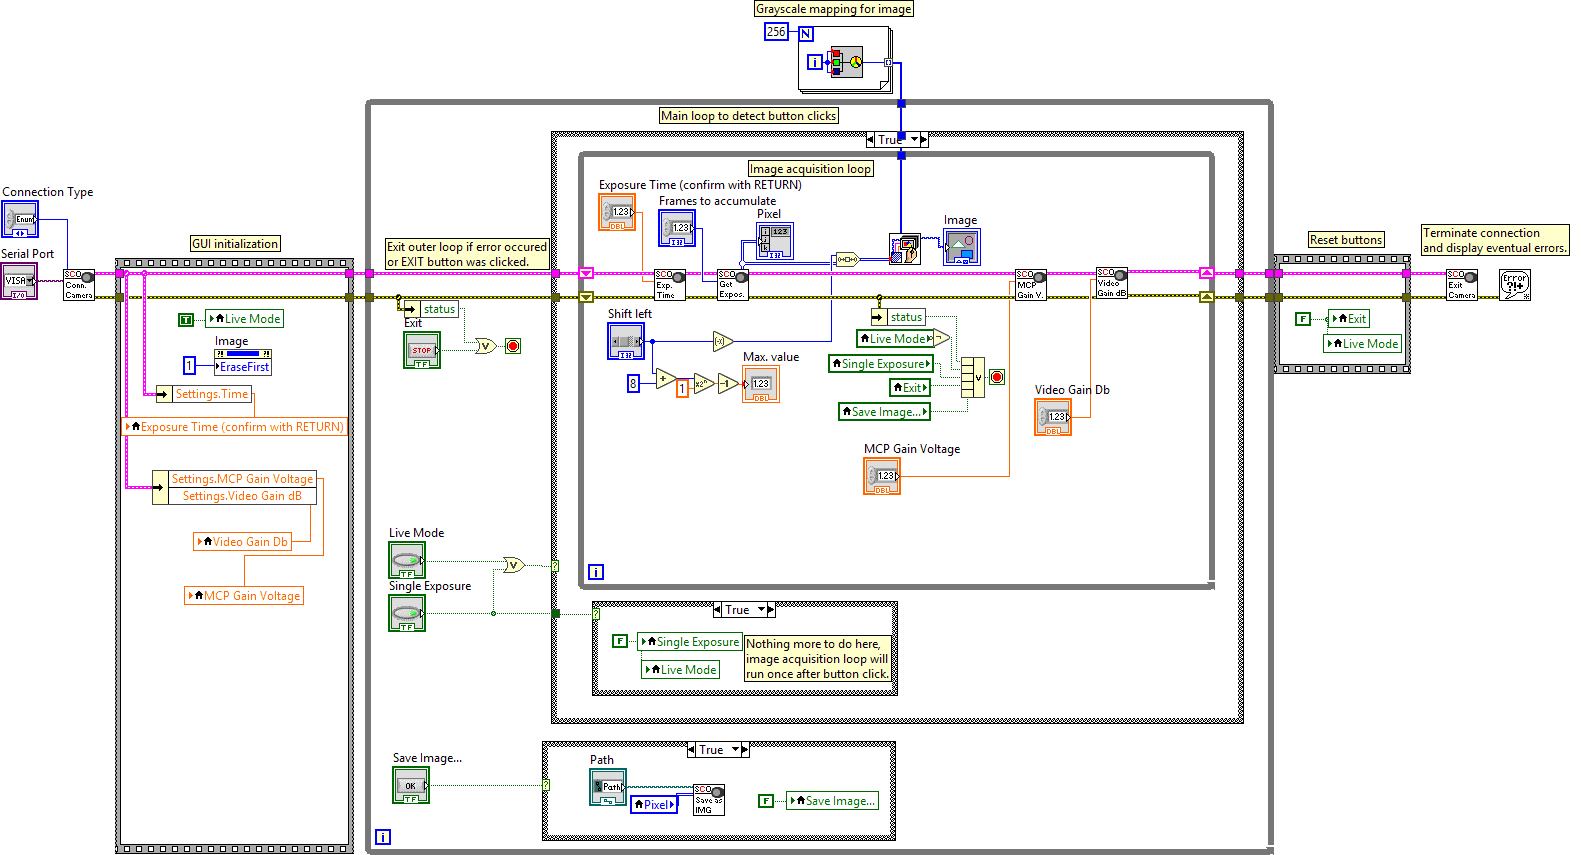
\includegraphics[width=\linewidth]{img/SCOexample_bd.png}
	\caption{Block Diagram del progetto per sola fotocamera}
	\label{fig:midProj_camera_bd}
\end{figure}
Si pu� considerare il bock diagram, in figura \ref{fig:midProj_camera_bd}, idealmente diviso in tre parti che eseguono in senquenza: una parte iniziale di inizializzazione, una intermedia di funzionamento del programma, e una finale di chiusura graceful dell'applicazione.\\
Il primo subVI invocato � \emph{ConnectCamera.vi} e deve essere invocato prima che la fotocamera sia utilizzata, imposta la connessione della fotocamera dipendentemente dall'input immesso dall'utente; restituisce in uscita un cluster contenente tutte le informazioni che riguardano le impostazioni della fotocamera. Tale cluster di dati, insieme al cluster di errore, entra in una flat sequence che recupera le impostazioni memorizzate da un uso antecedente dello strumento e le mostra nel controlli appositi nel front panel; viene anche impostato il bottone booleano \textit{Live Mode} a false.\\
In seguito alla flat sequence troviamo un ciclo while con lo scopo di individuare il cambiamento dei bottoni e dei controlli. All'interno di questo ciclo sono presenti due case structure: la prima associata al bottone \textit{Save Image...} che permette di salvare l'immagine, la seconda associata all'\textit{or} fra il valore dei due bottoni \textit{Single Exposure} e \textit{Live Mode}. Viene eseguito quindi il codice all'interno di quest'ultima case structure qualora o un bottone o l'altro esclusivamente (grazie ad un'altra case structure interna) abbiamo il valore true. Una volta dentro la case structure viene eseguito un ciclo while all'interno del quale vengono invocate alcune API LabVIEW della fotocamera: dapprima \emph{SetExposureTime.vi} con la quale si setta il tempo di esposizione, poi \emph{GetExposure.vi} che restituisce la matrice di pixel corrispondente alla foto. Attraverso alcuni calcoli che tengono in considerazione anche il valore di fondo scala inserito viene generata l'immagine da visualizzare del controllo destinato. Il ciclo while interno si arresta se viene presa una singola immagine, oppure se non si � selezionata la modalit� Live Mode, o se si � premuto il bottone \textit{Exit} per uscire dal ciclo o quello di salvataggio dell'immagino, o ancora se si � verificato qualche errore. Il ciclo esterno si arresta invece se si � verificato qualche errore o se si � invocato il bottone \textit{Exit} per fermarlo.\\
All'esterno di tale ciclo viene eseguito l'ultimo frammento di codice: in una flat sequence vengono resettati i bottoni di \textit{Exit} e \textit{Live Mode}, impostandoli a false, e infine viene invocato l'ultimo subVI relativo alla fotocamera, \emph{ExitCamera.vi}, che ha il compito di rilasciare le risorse impegnate dal programma e arrestare la fotocamera nel modo corretto.

\section{Monocromatore}
Ad un primo tentativo di refactoring del progetto preesistente il codice relativo al controllo del monocromatore si � rivelato troppo caotico e sparso. Per questo si � realizzato un nuovo programma, prendendo ovviamente spunto dal precedente, dedicato solo al monocromatore, che rispettasse il corretto flusso dei dati e non facesse uso di flat sequence. Si descrivono di seguito front panel e block diagram di tale programma \cite{monoAPIManual}.

\subsection{Front Panel}
\begin{figure} [h]
	\centering
	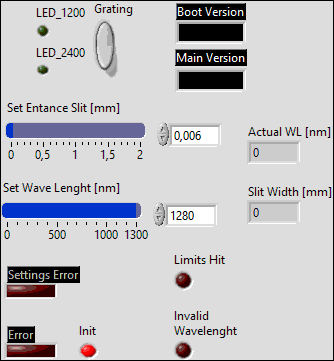
\includegraphics[width=0.5\linewidth]{img/ControlOnlyMono_Refactored.png}
	\caption{Front Panel del progetto per solo monocromatore}
	\label{fig:midProj_mono_fp}
\end{figure}
Gli elementi presenti nel front panel in figura \ref{fig:midProj_mono_fp} sono gli stessi dedicati al monocromatore nel precedente progetto, li rivedremo comunque brevemente. I controlli presenti sono:
\begin{itemize}
	\item \textit{Grating} per distinguere il tipo ti grating (1200 o 2400)
	\item \textit{Set Entrance Slit} per impostare la slit di entrata
	\item \textit{Set Wave Length} per inserire la lunghezza d'onda desiderata
\end{itemize}
Mentre gli indicatori sono:
\begin{itemize}
	\item \textit{Init} led che segnala se il monocromatore � stato inizializzato correttamente
	\item \textit{Error} led che segnala la presenza di eventuali errori in fase di inizializzazione
	\item \textit{Boot/Main Version} informazioni sulla versione del programma in uso
	\item \textit{Actual WL} lunghezza d'onda effettiva inserita
	\item \textit{Slit Width} slit di entrata inserita
	\item \textit{Settings Error} led che segnala un eventuale errore generico nel settaggio delle impostazioni del monocromatore
	\item \textit{Limits Hit} led che segnala l'inserimento di una lunghezza d'onda troppo alta
	\item \textit{Invalid Wavelength} led che segnala l'inserimento di una lunghezza d'onda non valida
\end{itemize}

\subsection{Block Diagram}
\begin{figure} [h]
	\centering
	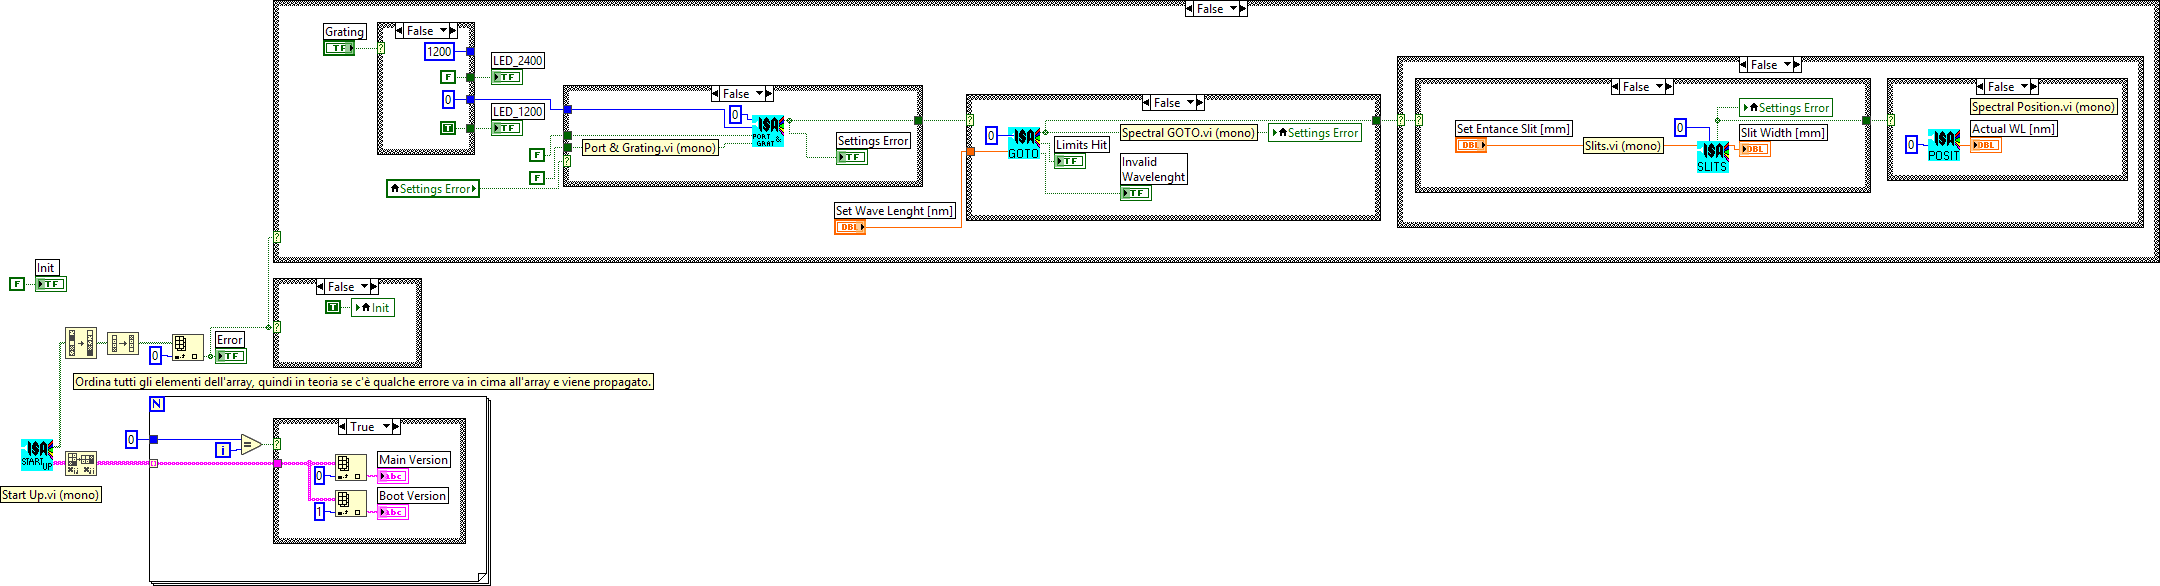
\includegraphics[width=\linewidth]{img/ControlOnlyMono_Refactored_bd.png}
	\caption{Block Diagram del progetto per solo monocromatore}
	\label{fig:midProj_mono_bd}
\end{figure}
Per la realizzazione del block diagram in figura \ref{fig:midProj_mono_bd} si � chiaramente preso spunto da quello gi� esistente, ma si � impiegato un consistente refactoring in particolare per eliminare le flat sequence.\\
Il primo subVI ad essere invocato � \emph{Start Up.vi} che porta i componenti interni del monocromatore nella posizione di default e restituisce il numero di versione del programma. Tale subVI restituisce anche un array di errori: esso viene ordinato in ordine crescente e ne viene estratto l'elemento in cima, se vi � un errore allora non � possibile continuare con il programma, in caso contrario si pu� procedere. Si entra quindi (in assenza di errori) nella case structure che permette di impostare come si desidera il monocromatore. I subVI che vengono invocati, in sequenza, sono: \emph{Port \& Grating.vi} per specificare il grating, \emph{Spectral GOTO.vi} per portare gli elementi interni alla lunghezza d'onda inserita dall'utente, \emph{Slits.vi} per inserire la slit di entrata e \emph{Spectral Position.vi} per completare gli indicatori corrispondenti. Chiaramente ognuno di questi subVI � inserito all'interno di una case structure e verrano eseguiti solo qualora il subVI precedente non abbia restituito in uscita errori. In questo modo si eliminano completamente le flat sequence e si sfrutta l'andamento del flusso dei dati.
\chapter{Realizzazione del progetto}
\thispagestyle{empty}

Gli strumenti coinvolti nel progetto sono quelli descritti nei capitoli precedenti, il monocromatore Jobin-Yvon HR460, si veda la sottosezione \ref{subsec:descrizioneMonocromatoreStrumento}, e la fotocamera intensificata 4 Picos, accenno alla tecnologia della stessa nella sottosezione \ref{subsec:descrizioneFotocamera}. Di seguito si descrive il programma realizzato per il controllo dei due strumenti attraverso un unico programma.

\section{Approccio iniziale}
Avendo davanti un progetto gi� scritto e funzionante, anche se per una fotocamera diversa, il primo approccio � stato quello di cercare di integrare il vecchio programma sostituendo i subVI della fotocamera precedente con quelli della fotocamera attuale. Tale tentativo si � rivelato fin dall'inizio fallimentare in quanto il codice del vecchio progetto risulta troppo caotico e avviluppato per essere modificato senza operare ingenti cambiamenti. Si � quindi optato per una riscrittura completa del codice prendendo sempre spunto da quello gi� scritto per le parti riutilizzabili.

\section{Struttura del progetto}
\begin{figure} [h]
	\centering
	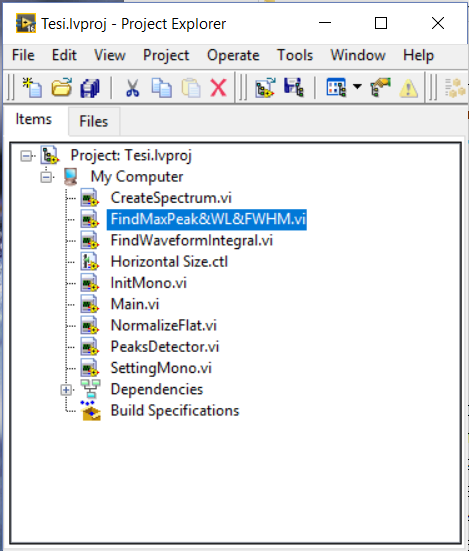
\includegraphics[width=0.5\linewidth]{img/Progetto.PNG}
	\caption{Struttura del progetto}
	\label{fig:newProj_lvproj}
\end{figure}
Per rendere il programma maggiormente organico e comprensibile si � deciso di creare un progetto LabVIEW: in questo modo i file e i subVI coinvolti sono raggruppati in un unico progetto (figura \ref{fig:newProj_lvproj}), che risulta sicuramente pi� gestibile di un semplice insieme di file.\\
Si � creato all'inizio un VI principale, un \emph{Main.vi} che ha lo stesso scopo dei \textit{main} degli altri linguaggi di programmazione. In seguito si � cercato di creare pi� subVI possibile per rendere il programma leggibile e ordinato. Si descriveranno pi� avanti i subVI contenuti nel progetto e i loro scopi.

\section{Front Panel}
La struttura pensata per il front panel di questo progetto � quella dell'interfaccia grafica a \textit{tab} (controllo grafico di navigazione che permette all'utente di muoversi da un gruppo di controlli a un altro). Tale widget permette un'ideale suddivisione delle diverse aree di competenza del programma: di seguito verranno elencate con una descrizione degli elementi contenuti in ognuna.
\begin{itemize}
\begin{figure} [h]
	\centering
	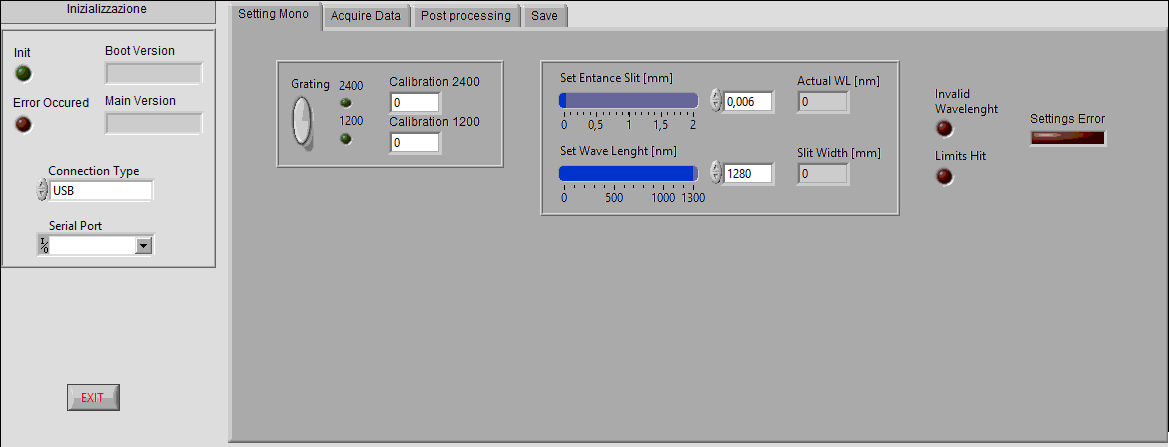
\includegraphics[width=\linewidth]{img/MainSettingMono.png}
	\caption{Front Panel del progetto, tab \textit{Setting Mono}}
	\label{fig:newProj_fp_SettingMono}
\end{figure}
	\item \textit{Setting Mono}, figura \ref{fig:newProj_fp_SettingMono}, contiene i controlli necessari al settaggio del monocromatore. \textit{Grating} per impostare il grating (1200 o 2400) e rispettivi controlli per specificarne un eventuale calibrazione. \textit{Set Entrance Slit} e \textit{Set Wave Length} per impostare la slit di entrata e la lunghezza d'onda. \textit{Actual WL} e \textit{Slit Width} per visualizzare lunghezza d'onda e slit effettivamente inserite. Sono presenti inoltre tre led: \textit{Settings Error} indica un errore generico di settaggio, \textit{Invalid Wavelength} indica l'inserimento di una lunghezza d'onda non valida e \textit{Limits hit} evidenzia l'inserimento di un valore oltre i limiti consentiti.
	\begin{figure} [h]
		\centering
	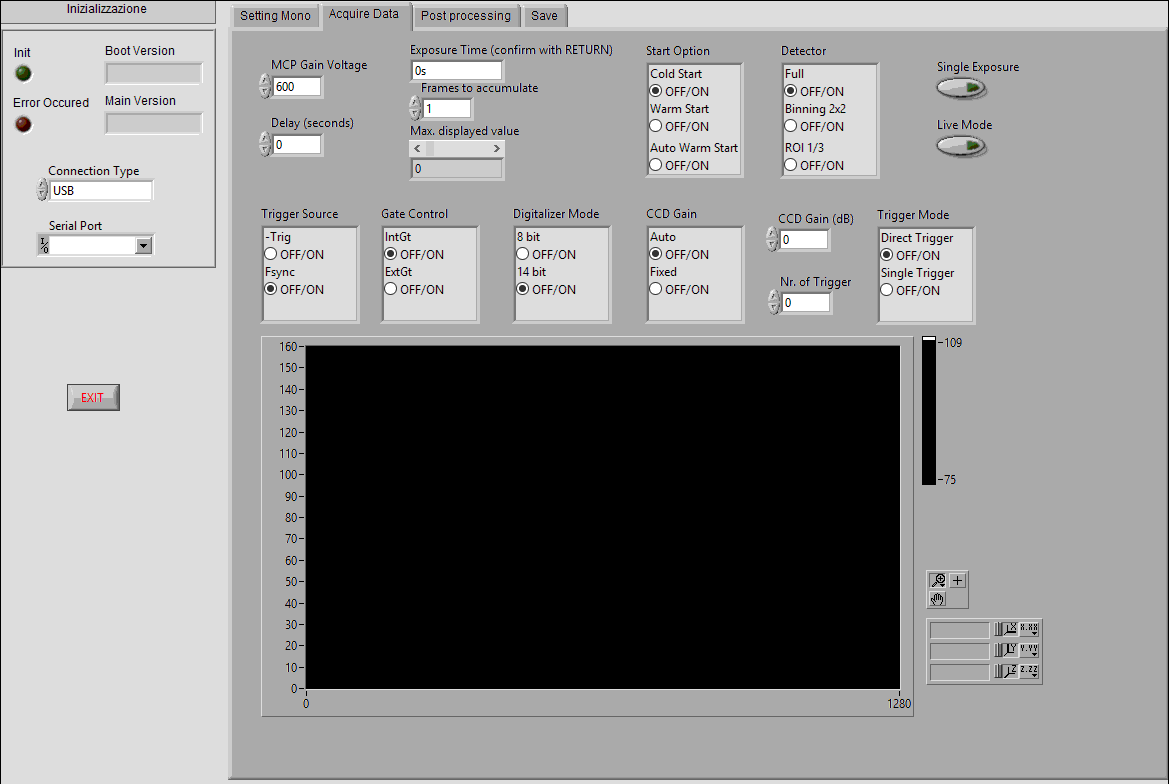
\includegraphics[width=\linewidth]{img/MainAcquireData.png}
	\caption{Front Panel del progetto, tab \textit{Acquire Data}}
	\label{fig:newProj_fp_AcquireData}
\end{figure}
	\item \textit{Acquire Data}, figura \ref{fig:newProj_fp_AcquireData}, contiene tutti i controlli per poter impostare la fotocamera e acquisire i dati.
\begin{figure} [h]
	\centering
	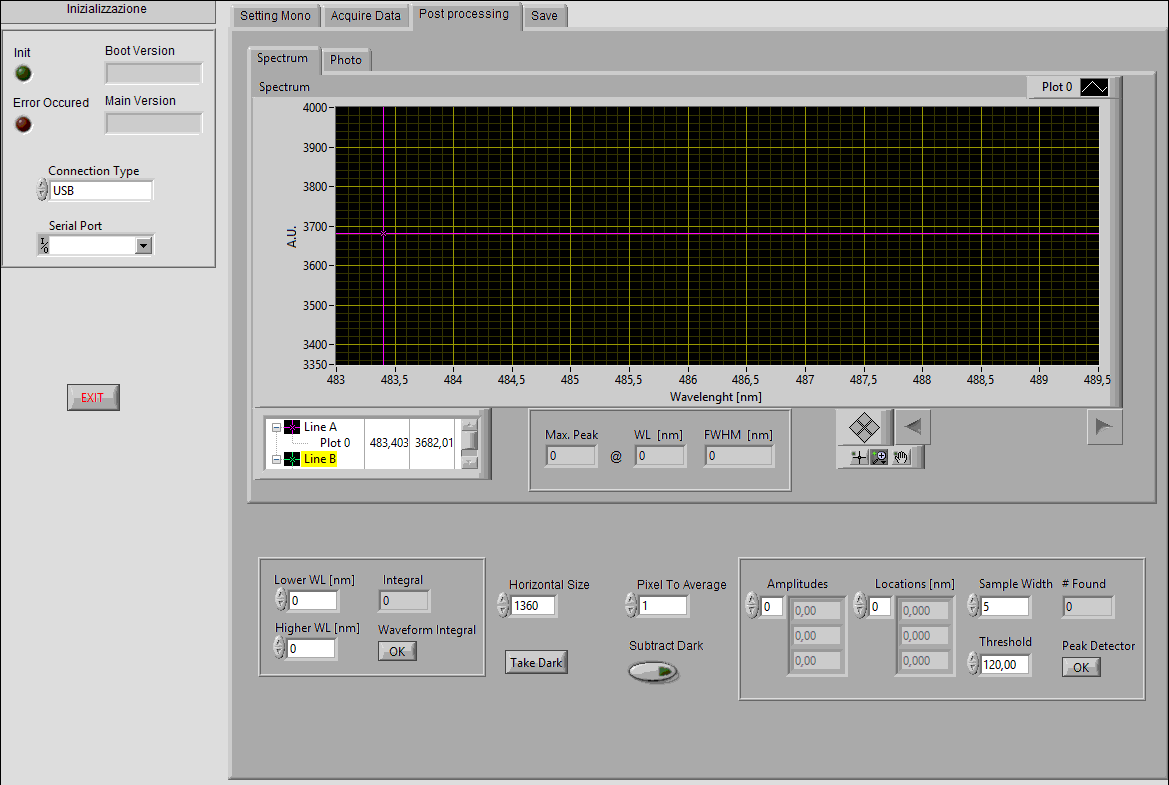
\includegraphics[width=\linewidth]{img/MainPostProc.png}
	\caption{Front Panel del progetto, tab \textit{Post Processing}}
	\label{fig:newProj_fp_PostProc}
\end{figure}
	\item \textit{Post Processing}, figura \ref{fig:newProj_fp_PostProc}, permette di visualizzare lo spettro corrispondente all'immagine acquisita ed effettuare dei calcoli su tali dati. Con \textit{Waveform Integral} � possibile calcolare l'integrale della lunghezza d'onda su un certo intervallo. \textit{Peak Detector} consente di visualizzare il numero di picchi trovati al di sopra di una certa soglia da inserire e i loro valori. Attraverso il controllo \textit{Pixel To Average} � possibile scegliere il numero di pixel da con cui fare la media da visualizzare poi nel grafico. Sono stati mantenuti anche i controlli per acquisire il background e sottrarlo alla foto.
	\begin{figure} [h]
		\centering
	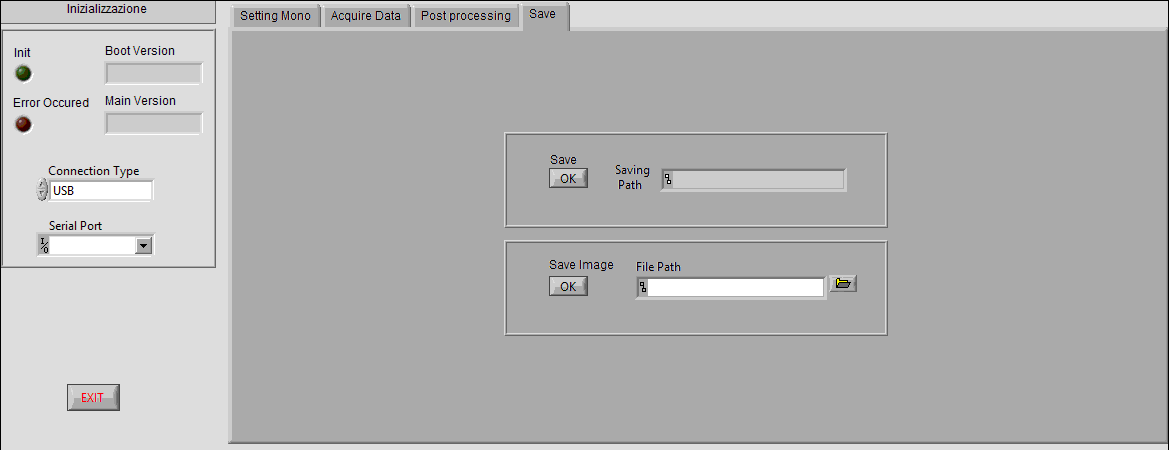
\includegraphics[width=\linewidth]{img/MainSave.png}
	\caption{Front Panel del progetto, tab \textit{Save}}
	\label{fig:newProj_fp_Save}
\end{figure}
	\item \textit{Save}, figura \ref{fig:newProj_fp_Save}, presenta due controlli booleani: \textit{Save} salva i dati ben formattati in un file di testo che pu� essere aperto successivamente con altri editor, \textit{Save Image} salva invece l'immagine vera e propria.
\end{itemize}
Al di fuori di questo controllo � presente un pannello dedicato all'inizializzazione degli strumenti. Il led \textit{Init} segnala che il monocromatore � stato inizializzato senza errori e viene visualizzata anche la versione del programma, in caso contrario si attiva il led \textit{Error Occured}. Sono presenti anche due controlli per specificare la connessione che si intende utilizzare verso la fotocamera: \textit{USB} per connetterla al calcolatore attraverso cavo USB, \textit{CameraLink} o \textit{Analog} per altre modalit� di connessione non contemplate in questo progetto.\\
Infine il bottone \textit{Exit} consente di arrestare il programma nel modo corretto rilasciando le risorse impiegate.

\section{Block Diagram}
\begin{figure} [h]
	\centering
	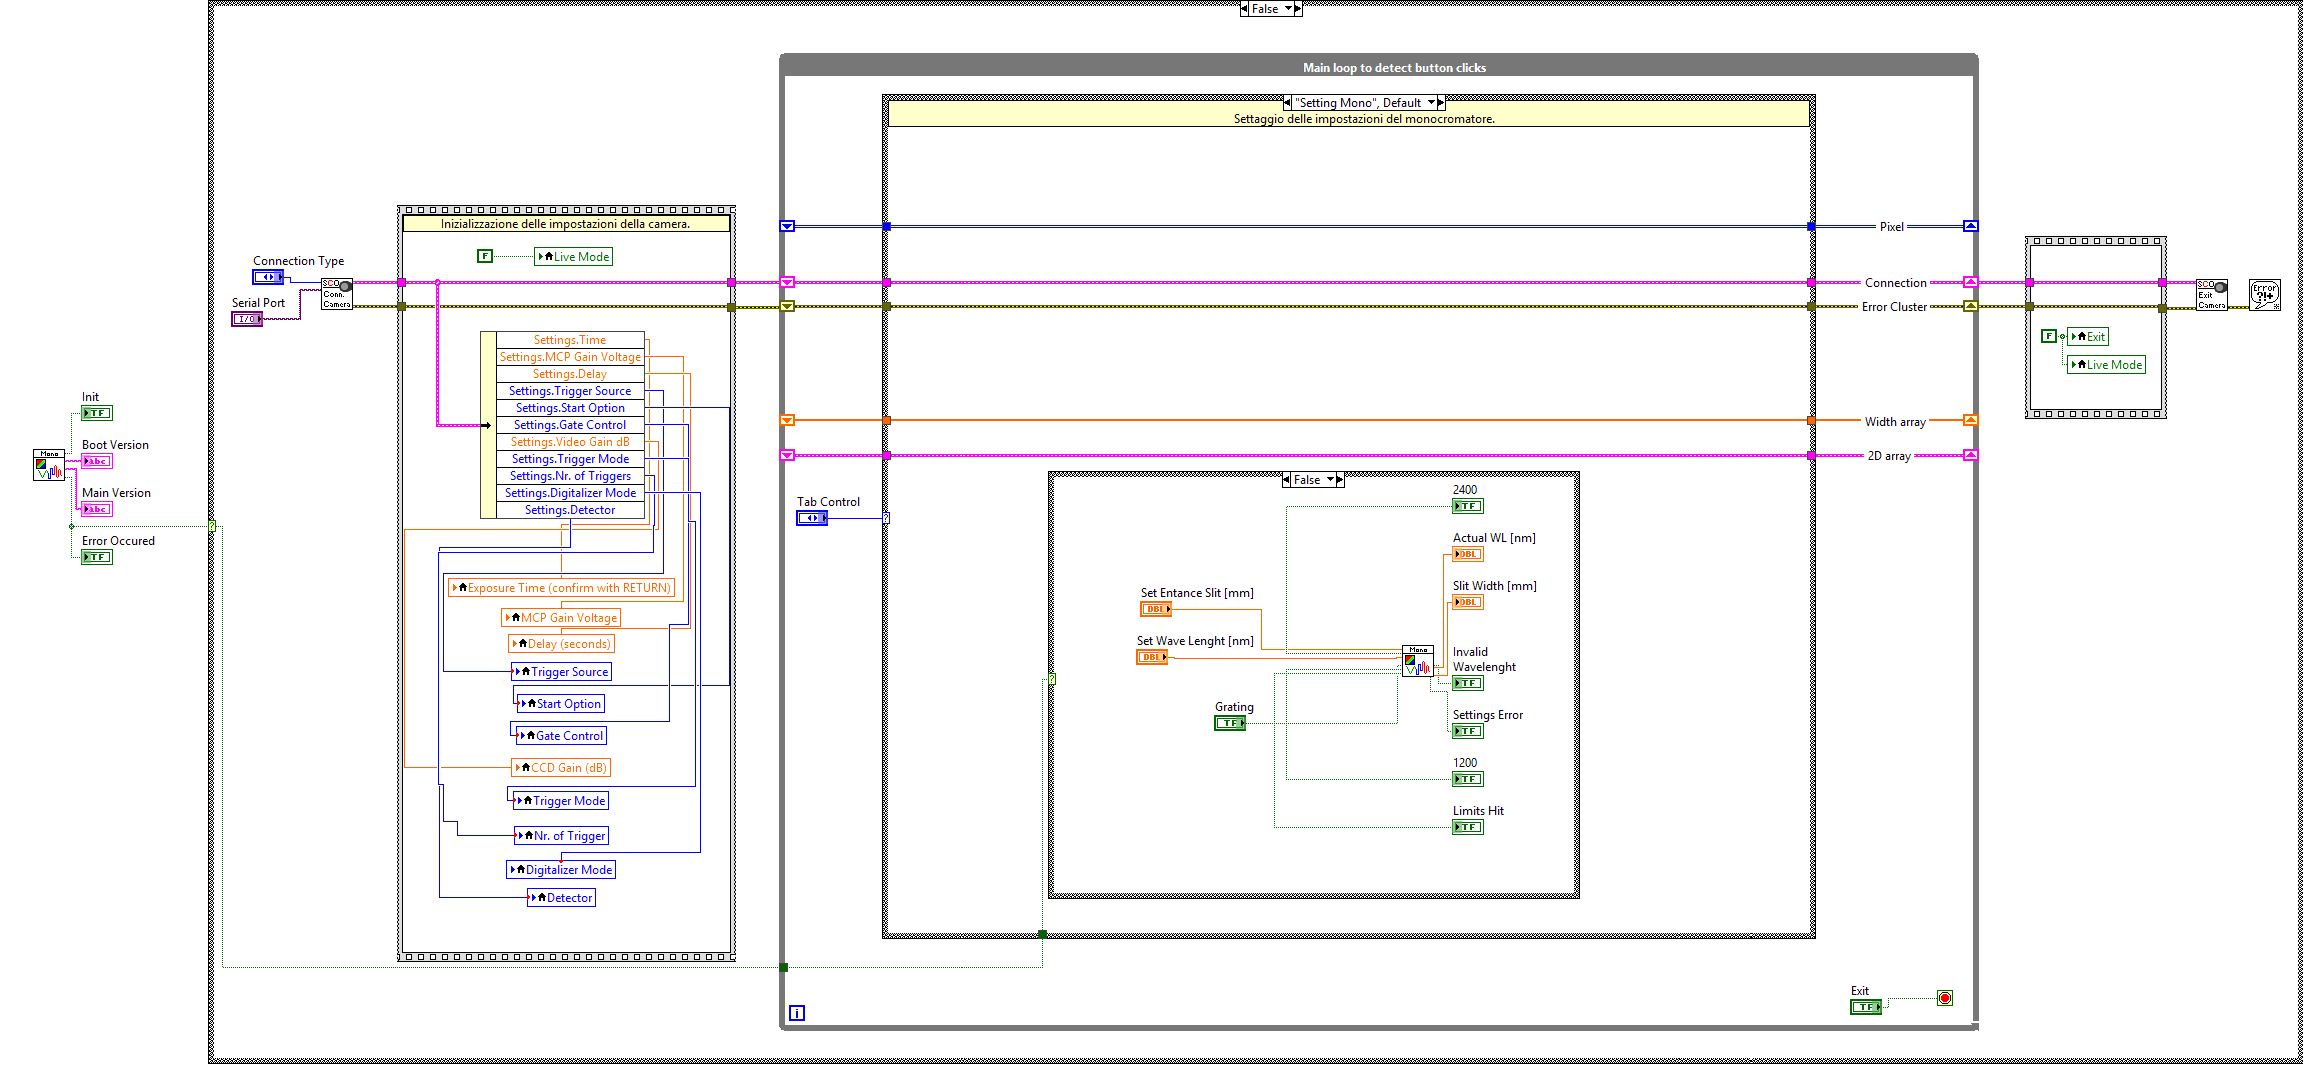
\includegraphics[width=\linewidth]{img/Main_bd.png}
	\caption{Block Diagram del progetto}
	\label{fig:newProj_bd}
\end{figure}
Come detto sopra il programma � stato organizzato in un progetto che raggruppa tutti i subVI creati nel corso della scrittura del codice. Partendo dal VI principale \emph{Main.vi} si descrive il block diagram delineando poi nello specifico i singoli subVI.\\
Il primo subVI che viene eseguito � \emph{InitMono.vi} che, come si pu� intuire dal nome, ha il compito di inizializzare il monocromatore; solo se tale subVI esegue restituendo nessun errore � possibile continuare con il resto del programma, del resto non avrebbe senso se lo strumento che deve generare il soggetto delle immagini non funzionasse correttamente. Se quindi non ci sono errori in fase di inizializzazione del monocromatore si entra in una case structure che racchiude tutto il resto del programma: per prima cosa viene eseguito il subVI di connessione alla fotocamera \emph{ConnectCamera.vi} il cui output entra poi in una flat sequence atta a visualizzare le impostazioni della fotocamera inserite l'ultima volta che � stata utilizzata. Successivamente si entra in un ciclo while per rilevare le azioni dell'utente; all'interno di questo ciclo si trova una case structure legata al \textit{tab control} che permette alla struttura di discriminare il codice in base alla tab selezionata dall'utente. La scelta di tale schema prende spunto dal design pattern di macchina a stati finiti: non � presente un enumerativo e non c'� una vera e propria sequenza che viene eseguita, ma lo schema generale ricorda tale pattern. Analizziamo quindi il codice eseguito nei quattro frame:
\begin{description}
\item[Setting Mono] Figura \ref{fig:newProj_bd}. All'interno di un'ulteriore case structure viene eseguito il subVI \emph{SettingMono.vi}, si faccia riferimento al codice descritto nella sezione \ref{sec:monocromatore_proj_singolo}.
\begin{figure} [h]
	\centering
	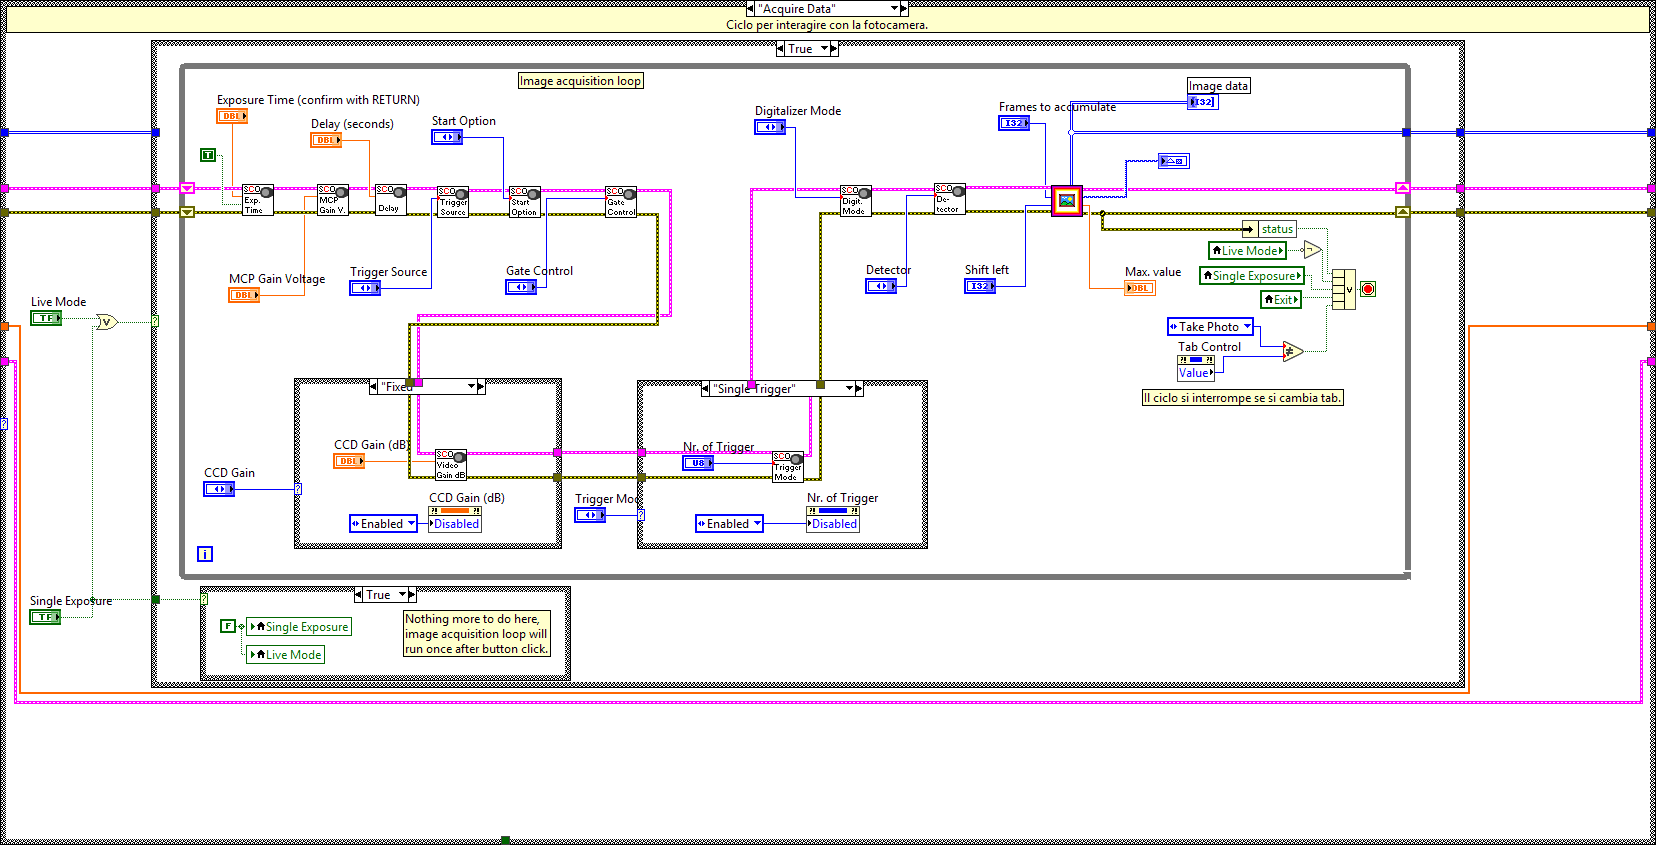
\includegraphics[width=\linewidth]{img/Main_acquireData.png}
	\caption{Block Diagram del progetto, frame ``Acquire Data''}
	\label{fig:newProj_bd_acquire}
\end{figure}
\item[Acquire Data] Figura \ref{fig:newProj_bd_acquire}. Per questo frame della case structure si � scelto di non creare subVI in quanto le variabili di input e output sarebbero state troppo numerose e avrebbero reso il codice incomprensibile. Viene quindi eseguito il codice per l'acquisizione delle immagini (si fa riferimento a quello spiegato nella sezione \ref{sec:fotocamera_proj_singolo}). Il ciclo per l'acquisizione viene arrestato anche se viene selezionata dall'utente un'altra tab.
\begin{figure} [h]
	\centering
	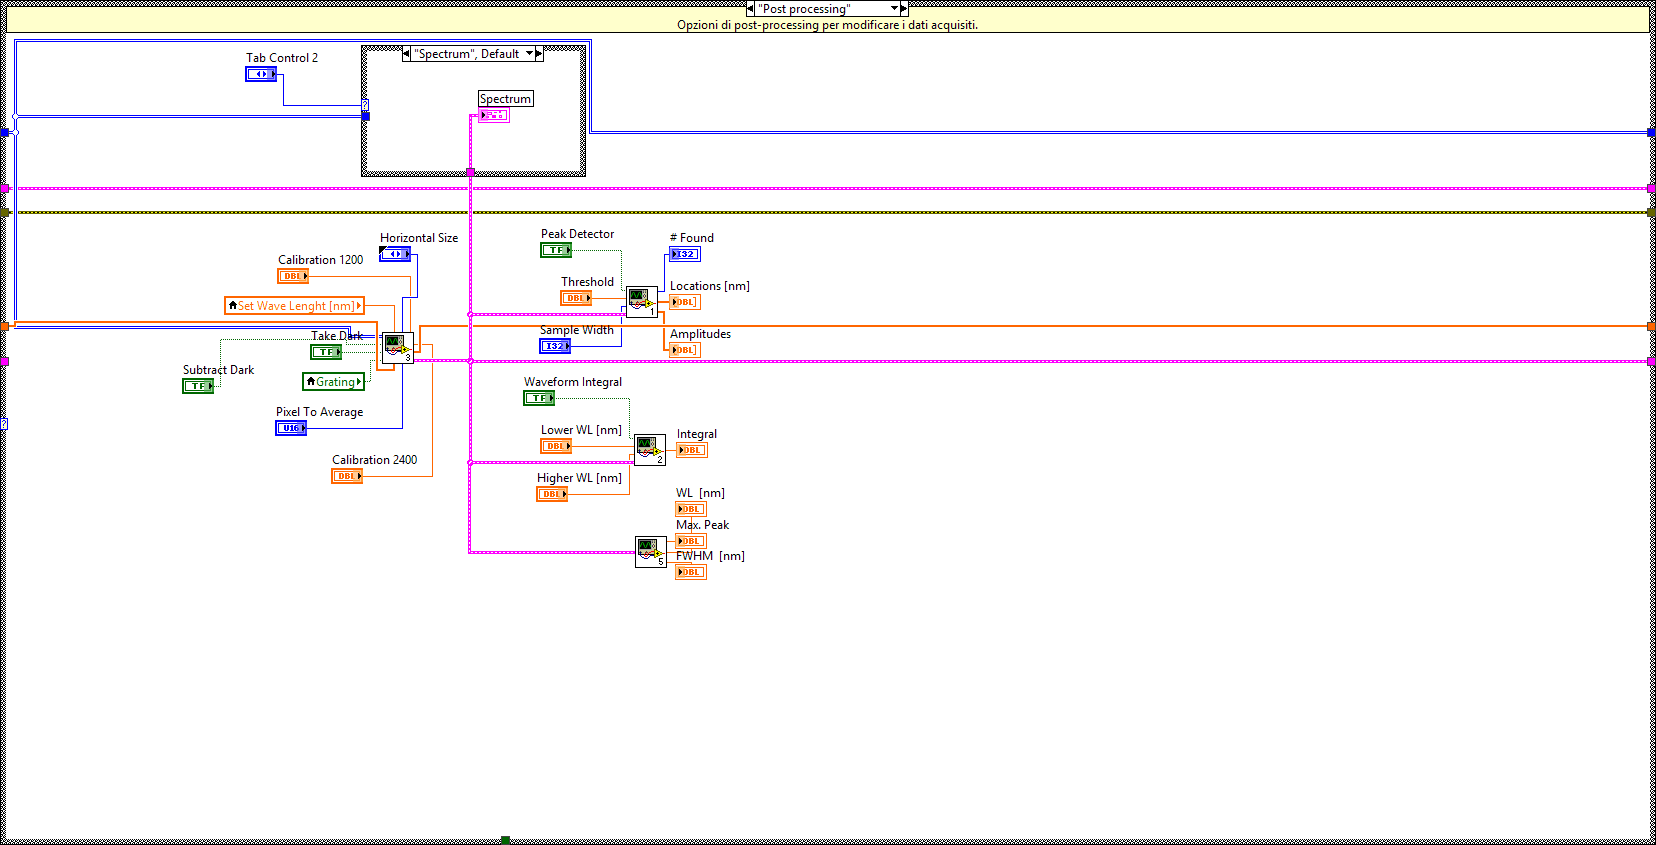
\includegraphics[width=\linewidth]{img/Main_postProc.png}
	\caption{Block Diagram del progetto, frame ``Post Processing''}
	\label{fig:newProj_bd_post}
\end{figure}
\item[Post processing] Figura \ref{fig:newProj_bd_post}. In questa frame sono stati inserite le elaborazioni sui dati che possono essere eseguite in seguito all'acquisizione dei dati. Abbiamo quindi una case structure che permette di visualizzare i dati come immagine o come spettro. Ci sono poi tre subVI: \emph{CreateSpectrum.vi} effettua i calcoli necessari per generare lo spettro da visualizzare, \emph{PeaksDetector.vi} restituisce i picchi sopra una certa soglia, \emph{FindWavefromIntegral.vi} calcola l'integrale su un intervallo della lunghezza d'onda.
\begin{figure} [h]
	\centering
	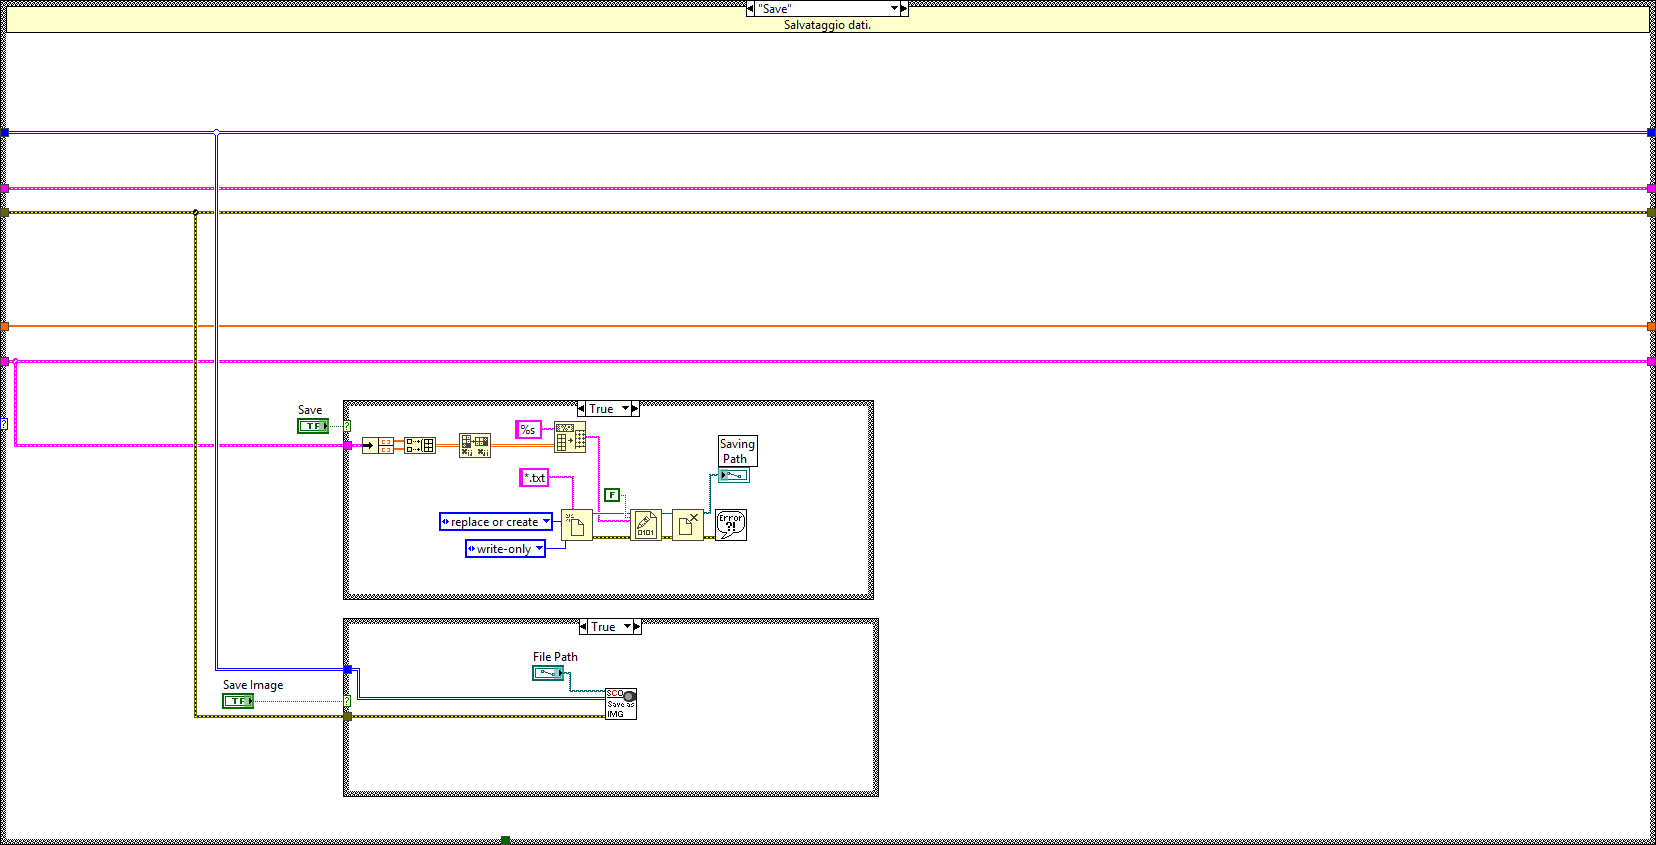
\includegraphics[width=\linewidth]{img/Main_save.png}
	\caption{Block Diagram del progetto, frame ``Save''}
	\label{fig:newProj_bd_save}
\end{figure}
\item[Save] Figura \ref{fig:newProj_bd_save}. Questo frame contiene due opzioni di salvataggio: \textit{Save} per salvare i dati in un file di testo, \textit{Save Image} per salvare l'immagine.
\end{description}
I shift register del ciclo esterno sono cinque: \textit{Pixel} contiene la matrice di pixel che compone l'immagine, \textit{Connection} contiene tutte le informazioni relative alla fotocamera, \textit{Error Cluster} riporta gli eventuali errori generati dalla fotocamera, \textit{Width Array} � l'array che contiene i valori delle lunghezze d'onda, \textit{2D Array} � la matrice con i valori da inserire nel grafico dello spettro.\\
Se infine viene arrestato il ciclo con il comando \textit{Exit}, viene eseguita l'ultima flat sequence che resetta i valori dei controlli di acquisizione delle immagini e viene eseguito anche il subVI \emph{ExitCamera.vi} per la chiusura graceful del programma e il rilascio delle risorse.

\subsection{Descrizione subVI}
Si descrivono di seguito i singoli subVI e le loro funzionalit�. Saranno analizzati solo i block diagram, in quanto i front panel hanno il solo scopo di mostrare input e output.
\begin{description}
\begin{figure} [h]
	\centering
	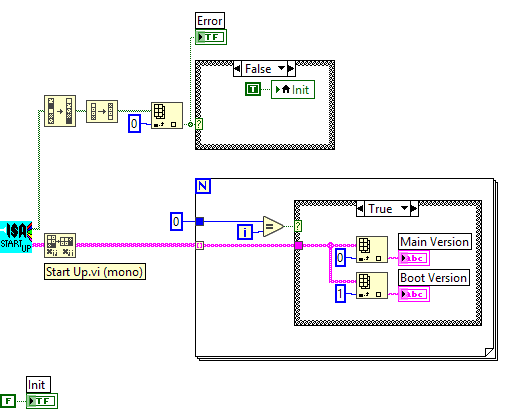
\includegraphics[width=\linewidth]{img/InitMonod.png}
	\caption{Block Diagram del subVI \emph{InitMono.vi}}
	\label{fig:newProj_bd_sub_initMono}
\end{figure}
\item[\textit{InitMono.vi}] Figura \ref{fig:newProj_bd_sub_initMono}. Il compito di questo subVI � quello di interrogare il monocromatore riportandolo al suo stato di default. Rispetto al codice presente nel progetto antecedente � stato leggermente modificato. Sono state eliminate tutte le flat sequence, che forzano il flusso logico dei dati. Dopo che � stato invocato il subVI del monocromatore \emph{Start Up.vi}, il led \textit{Init} viene impostato a true solo ed esclusivamente se non sono presenti errori nella matrice di errori restituita dallo stesso (si veda la sezione \ref{sec:monocromatore_proj_singolo}).
\begin{figure} [h]
	\centering
	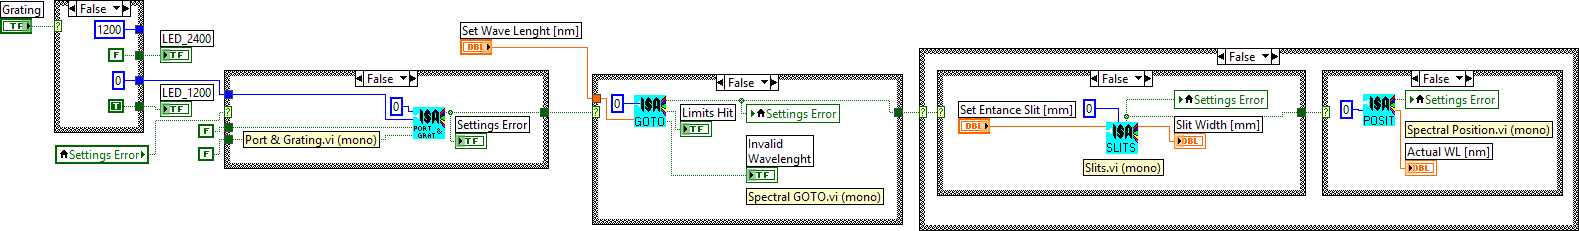
\includegraphics[width=\linewidth]{img/SettingMonod.png}
	\caption{Block Diagram del subVI \emph{SettingMono.vi}}
	\label{fig:newProj_bd_sub_settingMono}
\end{figure}
\item[\textit{SettingMono.vi}] Figura \ref{fig:newProj_bd_sub_settingMono}. Anche questo subVI � stato modificato rispetto al codice precedente eliminando tutte le flat sequence (si veda la sezione \ref{sec:monocromatore_proj_singolo}).
\begin{figure} [h]
	\centering
	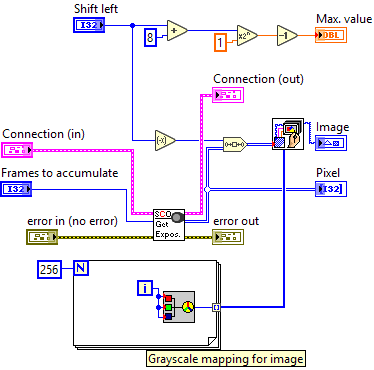
\includegraphics[width=0.6\linewidth]{img/CreateImaged.png}
	\caption{Block Diagram del subVI \emph{CreateImage.vi}}
	\label{fig:newProj_bd_sub_CreateImage}
\end{figure}
\item[\textit{CreateImage.vi}] Figura \ref{fig:newProj_bd_sub_CreateImage}. In seguito all'invocazione del subVI della fotocamera \emph{GetExposure.vi} viene invocata la funzione \emph{Draw Unflattened Pixmap.vi} per creare l'immagine vera e propria che possa essere visualizzata in un indicatore apposito.
\begin{figure} [h]
	\centering
	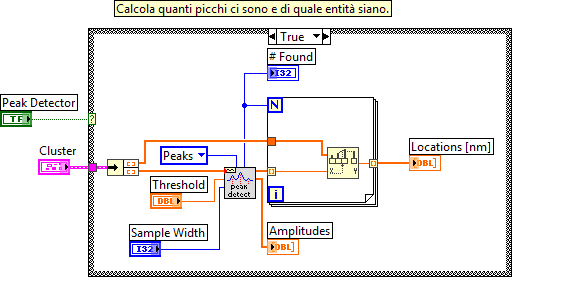
\includegraphics[width=\linewidth]{img/PeaksDetectord.png}
	\caption{Block Diagram del subVI \emph{PeaksDetector.vi}}
	\label{fig:newProj_bd_sub_PeaksDetector}
\end{figure}
\item[\textit{PeaksDetector.vi}] Figura \ref{fig:newProj_bd_sub_PeaksDetector}. Lo scopo di questo subVI � quello di trovare, attraverso la funzione \emph{Waveform Peak Detection.vi}, il numero di picchi presenti nella matrice in ingresso con rispettivi valori di lunghezza d'onda e intensit� del picco.
\begin{figure} [h]
	\centering
	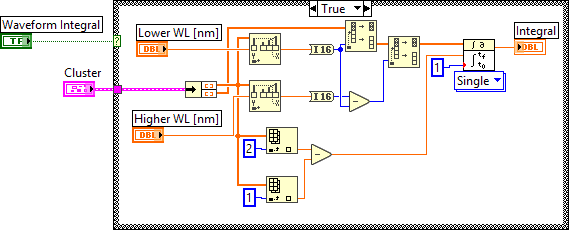
\includegraphics[width=\linewidth]{img/FindWaveformIntegrald.png}
	\caption{Block Diagram del subVI \emph{FindWaveformIntegral.vi}}
	\label{fig:newProj_bd_sub_FindWaveformIntegral}
\end{figure}
\item[\textit{FindWavefromIntegral.vi}] Figura \ref{fig:newProj_bd_sub_FindWaveformIntegral}. Data in ingresso la matrice con lunghezza d'onda e intensit� dello spettro, questo subVI calcola l'integrale, con apposite funzioni, su un intervallo in input.
\begin{figure} [h]
	\centering
	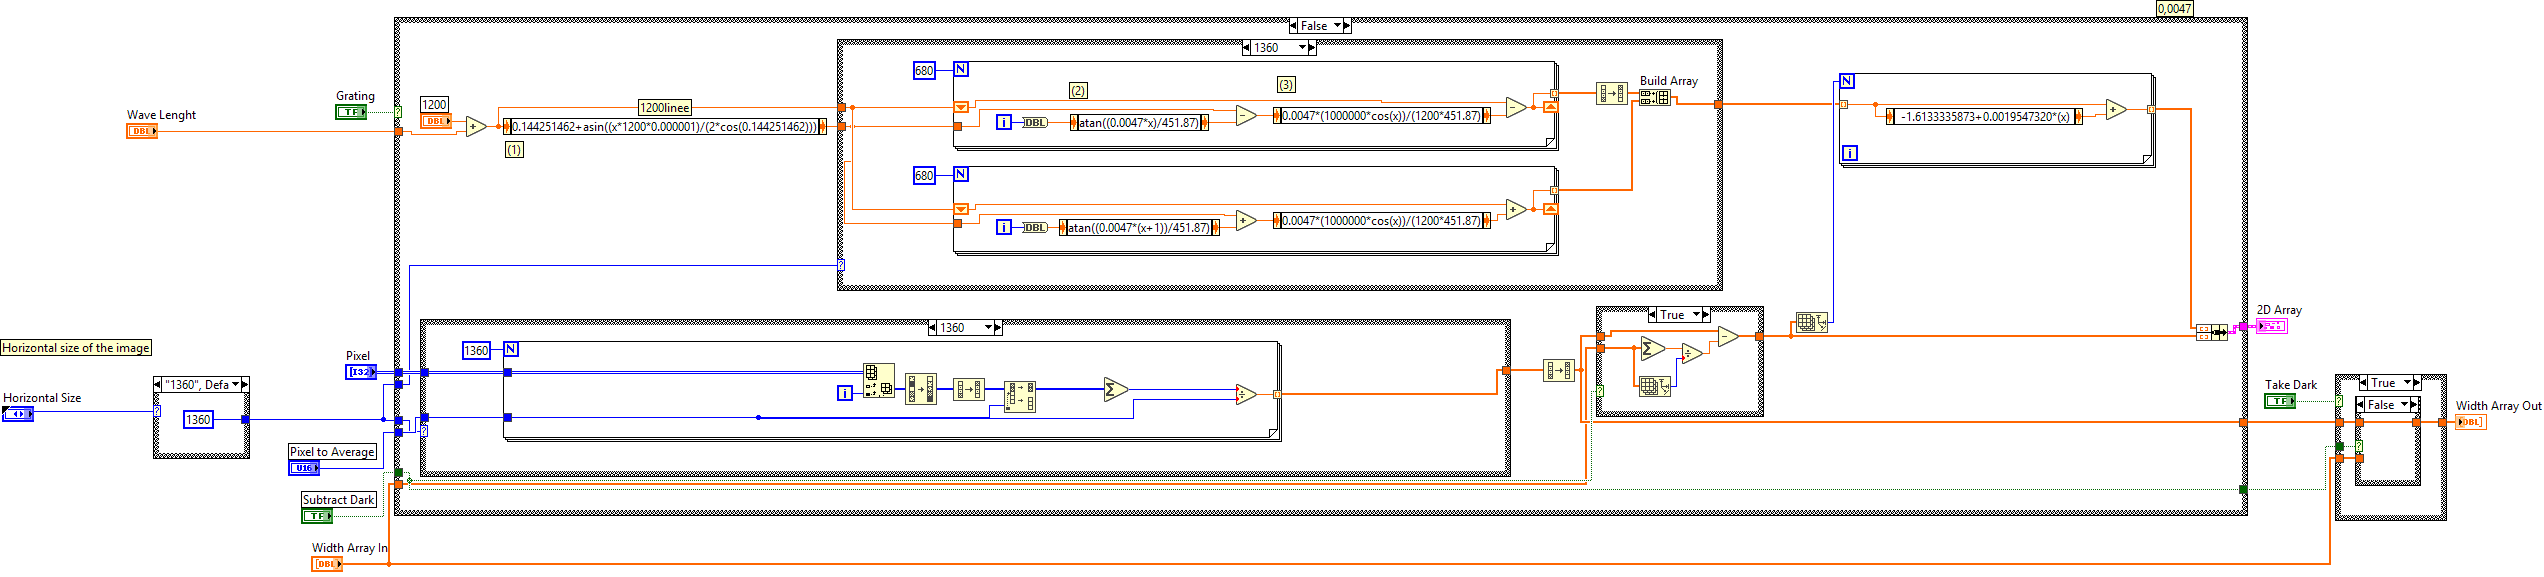
\includegraphics[width=\linewidth]{img/CreateSpectrumd.png}
	\caption{Block Diagram del subVI \emph{CreateSpectrum.vi}}
	\label{fig:newProj_bd_sub_CreateSpectrum}
\end{figure}
\item[\textit{CreateSpectrum.vi}] Figura \ref{fig:newProj_bd_sub_CreateSpectrum}. Come si pu� intuire dal nome, l'output di questo subVI consiste in una matrice di valori che rappresentano lunghezze d'onda con rispettiva intensit� dello spettro. I calcoli presenti sono stati riportati dal progetto precedente in quanto legati al monocromatore (si veda la sottosezione \ref{subsubsec:bdSpectra_secondBlock}). � stato modificato il valore del numero di pixel della larghezza dell'immagine (1360) e il valore di $w$ (0.0047).
\begin{figure} [h]
	\centering
	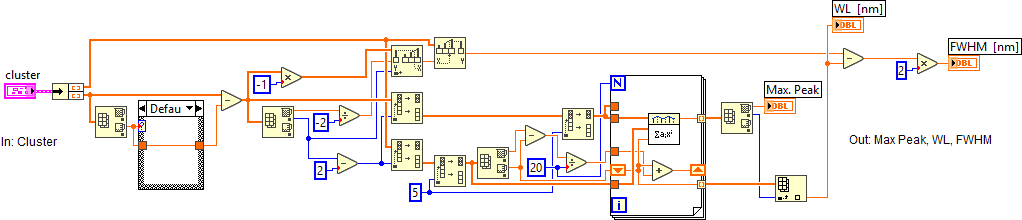
\includegraphics[width=\linewidth]{img/FindMaxPeakWLFWHMd.png}
	\caption{Block Diagram del subVI \emph{FindMaxPeak\&WL\&FWHM.vi}}
	\label{fig:newProj_bd_sub_FindMaxPeakWLFWHM}
\end{figure}
\item[\textit{FindMaxPeak\&WL\&FWHM.vi}] Figura \ref{fig:newProj_bd_sub_FindMaxPeakWLFWHM}. Questo subVI produce due risultati: restituisce il picco massimo e la sua corrispettiva lunghezza d'onda, e il valore della FWHM (Full Width at Half Maximum).
\end{description}
\begin{figure} [h]
	\centering
	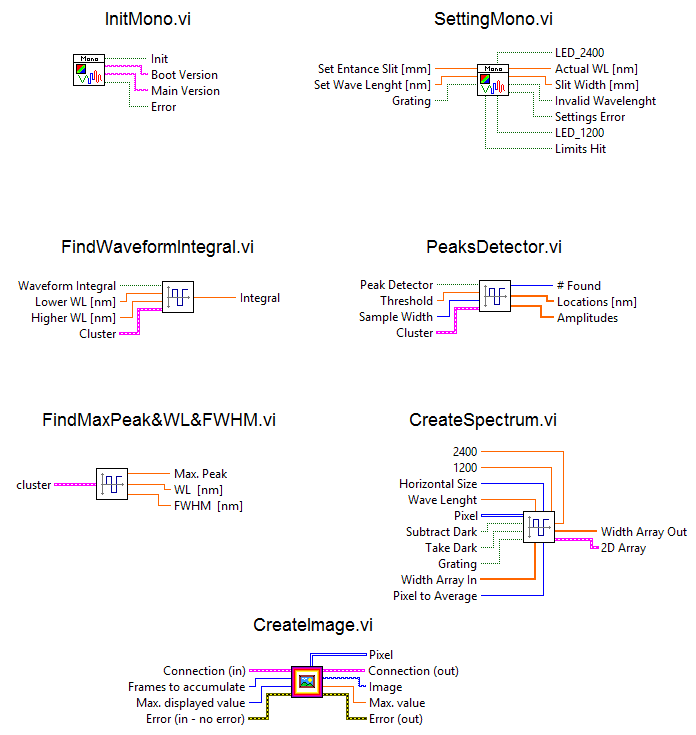
\includegraphics[width=\linewidth]{img/IconeSubVI.png}
	\caption{Icone dei subVI del progetto}
	\label{fig:newProj_bd_sub_icons}
\end{figure}
Nella figura \ref{fig:newProj_bd_sub_icons} si possono vedere le icone con input e output di tutti i subVI citati.

\section{Prova di utilizzo del programma}
Per provare l'effettivo funzionamento del programma, con l'ausilio di una lampada al mercurio e una fibra ottica, abbiamo fotografato lo spettro del mercurio. Dopo aver settato il monocromatore a $365nm$ di lunghezza d'onda, grating $2400$ e slit di entrata $0.6mm$, e la fotocamera con $3ms$ di tempo di esposizione e $820V$ di MCP Gain, abbiamo acquisito un'immagine.\\
\begin{figure} [h]
	\centering
	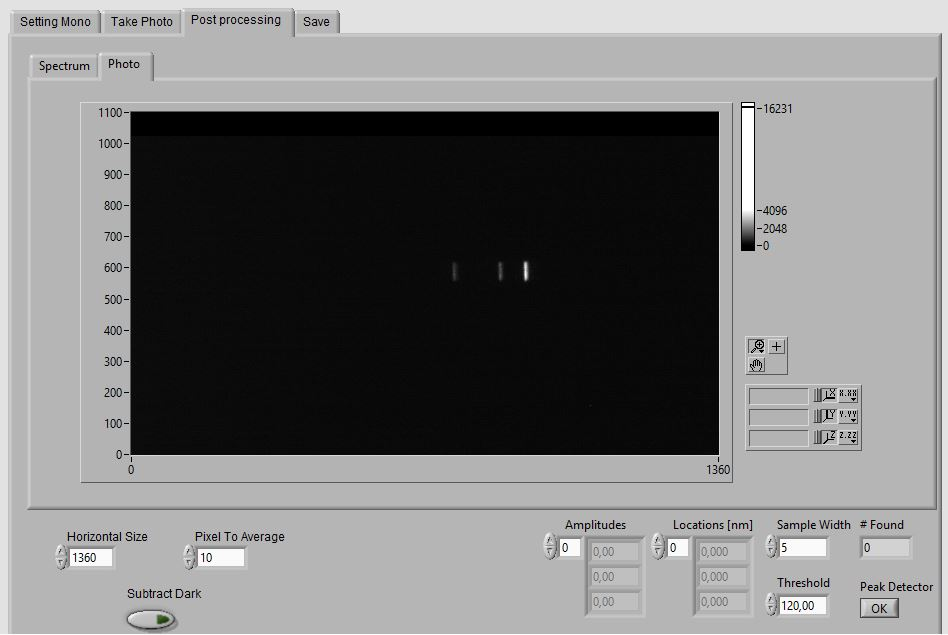
\includegraphics[width=\linewidth]{img/ProvaPhoto.JPG}
	\caption{Immagine dello spettro del mercurio acquisita con il progetto realizzato}
	\label{fig:newProj_try_photo}
\end{figure}
Nella figura \ref{fig:newProj_try_photo} si possono vedere tre linee bianche di intensit� decrescente che rappresentano lo spettro del mercurio; tale spettro si pu� vedere nella figura \ref{fig:newProj_try_spectrum} che mostra il grafico ottenuto dall'immagine. Lo spettro � formato da tre picchi, di cui uno di maggiore intensit� rispetto agli altri due, e corrispondono alle tre linee che compaiono nell'immagine.
\begin{figure} [h]
	\centering
	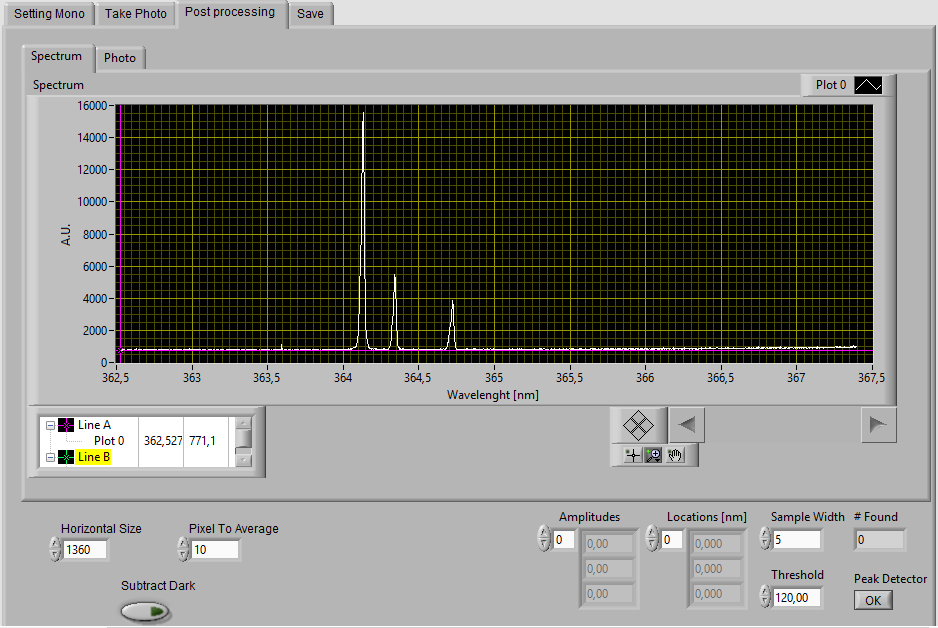
\includegraphics[width=\linewidth]{img/ProvaSpectrum.png}
	\caption{Spettro del mercurio processato a partire dall'immagine acquisita con il progetto realizzato}
	\label{fig:newProj_try_spectrum}
\end{figure}

\chapter{Conclusioni}
\thispagestyle{empty}

È stato realizzato il codice per il progetto richiesto: interfaccia grafica di controllo per una fotocamera intensificata e un monocromatore in ambiente LabVIEW. Per poter realizzare il programma è stata molto utile la partecipazione ad un corso su tale linguaggio per avere una conoscenza accademica oltre che concreta; tale corso ha anche permetto di conseguire la certificazione base di CLAD, Certified LabVIEW Associate Developer. 

\section{Risultati ottenuti}
Quasi tutte le specifiche richieste sono state soddisfatte. Il programma controlla correttamente entrambi gli strumenti e permette di salvare i dati acquisiti. Il monocromatore può essere settato correttamente controllando i dati prima di inviarli allo strumento, evitando così di danneggiare lo strumento. Per la fotocamera sono state riprese quasi tutte le opzioni presenti nel software proprietario. Nella fase di post processing dell'immagine è possibile visualizzare gli stessi calcoli presenti nel progetto preesistente.\\
La sottrazione del background deve ancora essere verificata in quanto la nuova fotocamera non dà la possibilità di acquisire un background, è necessario effettuare questa operazione manualmente. Rispetto al progetto preesistente è stato eliminato il comando di \textit{Normalize Flat} in quanto considerato poco rilevante al fine degli scopi di ricerca.

\section{Sviluppi futuri}
Il programma può senza dubbio essere migliorato, sia dal punto di vista del front panel che del block diagram. Per quanto riguarda il front panel si tratta di una questione prettamente estetica, che collide anche con la versione di LabVIEW installata sul calcolatore dal momento che non in tutte le versione di LabVIEW sono presenti gli stessi controlli e indicatori. Il block diagram si può considerare organico e comprensibile, è comunque sempre possibile aggiungere nuove funzionalità al programma, inclusa quella di \textit{Subtract Dark}. 

\clearpage{\pagestyle{empty}\cleardoublepage}

\begin{thebibliography}{90}             %crea l'ambiente bibliografia
\rhead[\fancyplain{}{\bfseries \leftmark}]{\fancyplain{}{\bfseries
\thepage}}
%%%%%%%%%%%%%%%%%%%%%%%%%%%%%%%%%%%%%%%%%aggiunge la voce Bibliografia
                                        %   nell'indice
\addcontentsline{toc}{chapter}{Bibliografia}
%%%%%%%%%%%%%%%%%%%%%%%%%%%%%%%%%%%%%%%%%provare anche questo comando:
%%%%%%%%%%%\addcontentsline{toc}{chapter}{\numberline{}{Bibliografia}}
\bibitem{K1} Primo oggetto bibliografia.
\bibitem{K2} Secondo oggetto bibliografia.
\bibitem{K3} Terzo oggetto bibliografia.
\bibitem{K4} Quarto oggetto bibliografia.
\end{thebibliography}
%%%%%%%%%%%%%%%%%%%%%%%%%%%%%%%%%%%%%%%%%non numera l'ultima pagina sinistra
\clearpage{\pagestyle{empty}\cleardoublepage}
\chapter*{Ringraziamenti}
\thispagestyle{empty}
Qui possiamo ringraziare il mondo intero!!!!!!!!!!\\
Ovviamente solo se uno vuole, non \`e obbligatorio.
\end{document}